\documentclass[a4paper,12pt]{report}

\newcommand{\nameInitial}{
    \textcolor{black}{S. Muller}  %change colour to black and enter your initial and surname
}
\newcommand{\nameFull}{
    \textcolor{black}{Sean Muller} %change colour to black and enter your firstname and surname
}
\newcommand{\stNumber}{
    \textcolor{black}{23575786} %change to black and enter your student number 
}
\newcommand{\myDate}{\textcolor{black}{\today} %change colour and if you want to date.
}
\newcommand{\signature}{frontmatter/fig/Signature}   %Upload your signature as "frontmatter/fig/Signature.png"


%%%%%%%%%%%%%%%%%%%%%%%%%%%%%%%%%%%%%%%%%%%%%%%%%%%%%%%%%%%%%%%%%
%From here you can ignore up to \begin{document} (line 107)
%%%%%%%%%%%%%%%%%%%%%%%%%%%%%%%%%%%%%%%%%%%%%%%%%%%%%%%%%%%%%%%%%
% Page layout
\usepackage[left=2.2cm,right=2.2cm,top=2.2cm,bottom=2.2cm]{geometry}
% Figures
\usepackage[margin=\the\parindent,small,bf,sf]{caption}
\usepackage{graphicx}
\usepackage{pdfpages}
\setlength{\abovecaptionskip}{7.5pt}  % spacing above and below captions
\newcommand*{\WaterMark}[2][0.2\paperwidth]{\AddToShipoutPicture*{\AtTextCenter{\parbox[c]{0pt}{\makebox[0pt][c]{\includegraphics[width=#1]{#2}}}}}}
\usepackage{subcaption}
% Font and text
\usepackage[afrikaans,english]{babel}
\usepackage{microtype}
\usepackage{setspace}
\usepackage{lmodern}
\newcommand{\myemph}[1]{{\sffamily\bfseries#1}}
\sloppy
\onehalfspacing
\usepackage{siunitx}
\usepackage{lipsum}
% Headings
\usepackage[raggedright,sf,bf]{titlesec}
\titlelabel{\thetitle.\ }
\titleformat{\chapter}[display]{\huge\bfseries\sffamily}{\chaptertitlename\ \thechapter}{15pt}{\raggedright}
% \titleformat{\chapter}[display]{\centering\huge\bfseries\sffamily}{\chaptertitlename\ \thechapter:}{15pt}{}
\titlespacing*{\chapter}{0pt}{0pt}{10pt}  % remove spacing before chapter headings
% Table of contents
\makeatletter
\let\originall@chapter\l@chapter
\def\l@chapter#1#2{\originall@chapter{{\sffamily #1}}{#2}}
\makeatother
\let \savenumberline \numberline
\def \numberline#1{\savenumberline{#1.}}
% Mathematics
\usepackage[cmex10]{amsmath}
\usepackage{amssymb}
\usepackage{cancel}
\DeclareMathOperator*{\argmax}{arg\,max}
\newcommand{\T}{^\textrm{T}}
\newcommand{\tr}{\textrm{tr}}
\renewcommand{\vec}[1]{\boldsymbol{\mathbf{#1}}}
\newcommand{\defeq}{\triangleq}
% Tables
\usepackage{booktabs}
\usepackage{tabularx}
\usepackage{multirow}
\newcommand{\mytable}{
    \centering
    \small
    \renewcommand{\arraystretch}{1.2}
    }
\renewcommand{\tabularxcolumn}[1]{m{#1}}
\newcolumntype{C}{>{\centering\arraybackslash}X}
\newcolumntype{L}{>{\raggedright\arraybackslash}X}
% Header and footer
\usepackage{fancyhdr}
\pagestyle{fancy}
\fancyhf{}
\renewcommand{\sectionmark}[1]{\markright{\normalsize \thesection.\ #1}}
\fancyhead[C]{\nouppercase{\textit{\rightmark}}}
\fancyhead[RO]{\thepage}
% \fancyhead[LE]{\thepage}  % double-sided printing
\fancyfoot{}
\setlength\headheight{14.5pt}
\renewcommand{\headrulewidth}{0pt}
\fancypagestyle{plain}{\fancyhead{}
                       \renewcommand{\headrulewidth}{0pt}
                       \fancyfoot[C]{\thepage}}
% Pseudo-code
\usepackage{algorithm}  % should go before \usepackage{hyperref}
% Table of contents and hyperlinks
\usepackage{hyperref}
\hypersetup{colorlinks=true,linktoc=all,citecolor=black,linkcolor=black}
\usepackage[nottoc]{tocbibind}
% Pseudo-code
\usepackage{algpseudocode}  % should go after \usepackage{hyperref}
\renewcommand{\thealgorithm}{\arabic{chapter}.\arabic{algorithm}} 
\captionsetup[algorithm]{labelfont={bf,sf},font=small,labelsep=colon}
% Bibliography
\usepackage{cite}  % automatically reorder inline citations
\bibliographystyle{IEEEtran}
% Fix titlesec issue
\usepackage{etoolbox}
\makeatletter
\patchcmd{\ttlh@hang}{\parindent\z@}{\parindent\z@\leavevmode}{}{}
\patchcmd{\ttlh@hang}{\noindent}{}{}{}
\makeatother
 \usepackage[normalem]{ulem}
%%%%%%%%%%%%%%%%%%%%%%%%%%%%%%%%%%%%%%%%%%%%%%%%%%%%%%%%%%%%%%%%%
% Ignore up to here. 
%%%%%%%%%%%%%%%%%%%%%%%%%%%%%%%%%%%%%%%%%%%%%%%%%%%%%%%%%%%%%%%%%

\begin{document}

% Front matter
\graphicspath{{frontmatter/fig/}}
\pagenumbering{Alph}

\begin{titlepage}
\begin{center}


\includegraphics[width=8cm]{frontmatter/fig/SU_logo_RGB_without_slogan.pdf}

\vfill

{\sffamily \bfseries \huge E344 Report \par}

\vfill

{\large {\Large \nameFull} \\ \stNumber \par}

\vfill

\vfill

{Report submitted in partial fulfilment of the requirements of the module \\
Design (E) 344 for the degree Baccalaureus in Engineering in the Department of
Electrical and Electronic Engineering at Stellenbosch University. \par}

\vfill

%{\large {Supervisor}: Dr L. Skywalker} %\\
% Department of Electrical and Electronic Engineering \par}

\vfill

{\Large \myDate}
\end{center}
\end{titlepage}

\pagenumbering{roman}
%\chapter*{Declaration}
\newpage
\pagestyle{plain}
\addcontentsline{toc}{chapter}{Declaration}
\makeatletter\@mkboth{}{Declaration}\makeatother

\centerline{
\includegraphics[width=8cm]{frontmatter/fig/SU_horizontal_RGB.pdf}}
\vspace*{-10pt}

\section*{\centering Plagiaatverklaring / \textit{Plagiarism Declaration}}

\vspace*{5pt}

\begin{enumerate}
    \item Plagiaat is die oorneem en gebruik van die idees, materiaal en ander intellektuele eiendom van ander persone asof dit jou eie werk is.\\
    \textit{Plagiarism is the use of ideas, material and other intellectual property of another's work
        and to present is as my own.}
    
    \item Ek erken dat die pleeg van plagiaat 'n strafbare oortreding is aangesien dit 'n vorm van diefstal is.\\
    \textit{I agree that plagiarism is a punishable offence because it constitutes theft.}
    
    \item Ek verstaan ook dat direkte vertalings plagiaat is. \\
    \textit{I also understand that direct translations are plagiarism.}
    
    \item Dienooreenkomstig is alle aanhalings en bydraes vanuit enige bron (ingesluit die internet) volledig verwys (erken). Ek erken dat die woordelikse aanhaal van teks sonder aanhalingstekens (selfs al word die bron volledig erken) plagiaat is. \\
    \textit{Accordingly all quotations and contributions from any source whatsoever (including the internet) have been cited fully. I understand that the reproduction of text without quotation marks (even when the source is cited) is plagiarism}
    
    \item Ek verklaar dat die werk in hierdie skryfstuk vervat, behalwe waar anders aangedui, my eie oorspronklike werk is en dat ek dit nie vantevore in die geheel of gedeeltelik ingehandig het vir bepunting in hierdie module/werkstuk of 'n ander module/werkstuk~nie. \\
    \textit{I declare that the work contained in this assignment, except where otherwise stated, is my original work and that I have not previously (in its entirety or in part) submitted it for grading in this module/assignment or another module/assignment.}
\end{enumerate}

\vfill

\noindent \begin{tabularx}{1.0\linewidth}{|L|L|}
    \hline
    \hspace{2cm} \large{\stNumber}& \vspace{4mm}\hspace{2cm} \includegraphics[height=1.5cm]{\signature}\\

    \vspace{0mm}{Studentenommer / \textit{Student number}} & \vspace{0mm} {Handtekening / \textit{Signature}} \\
    \hline
    \vspace{1mm}  \hspace{2cm} \large{\nameInitial} & \vspace{1mm} \hspace{2cm} \large{\myDate }\\
    \vspace{1mm} {Voorletters en van / \textit{Initials and surname}} & \vspace{1mm} {Datum / \textit{Date}} \\
    \hline
\end{tabularx}

\vspace{15pt}




\tableofcontents
\listoffigures
\listoftables
\chapter*{Nomenclature\markboth{}{Nomenclature }}
\addcontentsline{toc}{chapter}{Nomenclature}


\textcolor{red}{Update these lists to make it applicable to your project. It is in \texttt{/frontmatter/nomenclature.tex}}
% \vspace*{-3mm}
\subsubsection*{Variables and functions}
\textcolor{red}{Update this list to make it applicable to your project.}\\
\begingroup
\renewcommand{\arraystretch}{1.2}
\renewcommand{\tabularxcolumn}[1]{p{#1}}
\begin{tabularx}{\textwidth}{@{}p{2.5cm}L}
    $p(x)$ & Probability density function with respect to variable $x$.\\
    $P(A)$ & Probability of event $A$ occurring.\\
\end{tabularx}
\endgroup


%\newpage
\subsubsection*{Acronyms and abbreviations}


\textcolor{red}{Update this list to make it applicable to your project.}\\

\begingroup
\renewcommand{\arraystretch}{1.2}
\begin{tabular}{@{}p{2.5cm} l}
    AE      & Afrikaans English \\
    AID     & accent identification \\
\end{tabular}
\endgroup

\newpage
\pagenumbering{arabic}

% Contents
\chapter{Literature survey}\label{chap:Lit}

This chapter will cover a review on the different methods for current sensing and the limitations, considerations and configurations for operational amplifier design for current sensing. 

\section{Operational amplifiers}\label{sec:opamps}

\subsubsection{Operational amplifiers: limitations and considerations}\label{sec:opamps_limits}
limits that need to be considered for this specific use.
\subsubsection{Operational amplifier configurations}\label{sec:opamps_configs}
inverting
non-inverting
differential

\newpage
\section{Current sensing}\label{sec:cursens}
There are many different techniques to measure current. Both invasive and non invasive methods each with their own advantages and disadvantages that make them suitable for different situations. An invasive current sensor negatively affect the system and decreases performance whereas a non-invasive current sensor doesn't affect the operation of the system at a meaningful level. 

\subsubsection{Hall effect}\label{sec:cursens_hall}
The Hall effect current sensor is a non invasive method of current sensing that uses the magnetic field generated around a current carrying conductor \cite{CircuitDigest}. This magnetic field creates a voltage across the material of the sensor. Hall effect sensors measure this voltage to determine the current flowing in a conductor \cite{Hall}. There are many advantages to using a Hall effect sensor however, besides the amplifier circuit additional circuits are required and is more costly than other measurement methods \cite{CircuitDigest}.

\subsubsection{Rogowski coil}\label{sec:cursens_coil}
The Rogowski coil is a non invasive current sensing method that uses a helical shaped coil that is wrapped around the conductor that you want to measure current in. The coil outputs a voltage depending on the rate of change of current through the conductor, this requires an integrator circuit to create an output voltage that is proportional to the current. The Rogowski coil is very useful for high frequency currents and does not require complex temperature compensation. However this method is only suitable for AC current \cite{CircuitDigest}.

\subsubsection{Shunt Resistor}\label{sec:cursens_shunt}
The shunt resistor is the most common current sensing technique and uses a resistor in series with the current to be measured. This is a invasive current measuring method. The shunt resistor produces a voltage drop proportional to the current, however the resistance and hence the voltage must be kept low in order to reduce the power consumption. This requires a high gain amplifier circuit to increase the small voltages to meaningful levels. The shunt resistor is a very cost effective solution that works on both AC and DC however it creates a decrease in system efficiency and can't handle high currents due to power dissipation across the resistor. Thermal drift also results in error \cite{CircuitDigest}. 

High-side vs low-side current sensing is only applicable for invasive methods like the shunt resistor. Low-side has the advantages of being simple and low cost and low input common mode voltage however it can't detect high current due to a short \cite{EG_CurSens}. High-side current sensing removes the ground disturbance and can detect accidental shorts however it has a higher complexity and cost because the gain circuit must be able to handle high common mode voltages\cite{EG_CurSens}.  
\chapter{Detail design}\label{ch:detail_design}
%**********************************************
\section{Current sensor}\label{sec:current_sensor_design}
Currently being rewritten.
\subsection{Opamp configuration}\label{sec:config}


\subsection{Opamp design}
\begin{figure}
\centering
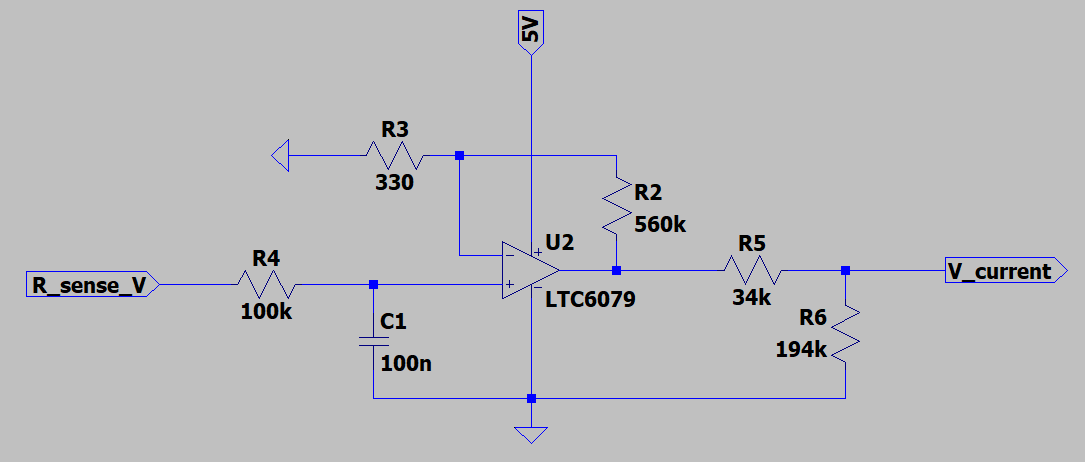
\includegraphics[width=0.65\linewidth]{./Figures/CurSens_SimCir.png}
\caption{Current sensing circuit design}
\label{fig:cursen_sim_cir}
\end{figure}

\newpage
\section{Analogue range sensor}
The HC-SR04 ultrasonic sensor requires a \SI{5}{\volt} supply and requires \SI{15}{\milli\ampere} to operate \cite{Design_SonicSens}. The frequency of the sensor output is the same as the input trigger frequency which is \SI{16}{\hertz}. Using a maximum distance of \SI{1}{\meter} and a minimum distance of \SI{5}{\centi\meter} results in a minimum duty cycle of 0.4\% and a maximum duty cycle of 10\%. The output pulses will have a maximum amplitude of  \cite{Design_SonicSens}.

Equation \ref{eqn:sens_gain} is used to calculate the needed gain of the system. In order to have the gain stage output a maximum of \SI{5}{\volt} at \SI{1}{\meter} a gain of 10.77 is required.

\begin{align}
Gain &= \frac{V_{Expected}}{V_{Duty Cycle \cdot V_{Amplitude}}}\label{eqn:sens_gain}
\end{align}

In order to determine the corner frequency fist the minimum attenuation must be calculated. The minimum attenuation can be calculated using the gain and amplitude of the first harmonic frequency component in the square wave to determine the size of the output ripple voltage, see Equation \ref{eqn:sens_harm}. Since the second harmonic and higher will all be attenuated more aggressively than the first harmonic it will contribute the most to the ripple voltage. 

\begin{align}
First Harmonic Amplitude &= V_{Amplitude} \cdot DutyCycle \cdot sinc(\pi \cdot DutyCycle)\label{eqn:sens_harm}\\
MinimumAttenuation &= 20log(\frac{MaximumNoise}{FirstHarmonicAmplitude \cdot Gain})\label{eqn:sens_atten}
\end{align}

Using Equation \ref{eqn:sens_atten} it is determined that an attenuation of atleast \SI{-41}{\decibel} is needed at \SI{16}{\hertz}. The corner frequency is then determined solving a simple straight line graph equation as shown in Equation \ref{eqn:sens_cutoff}.

\begin{align}
log(w) &= \frac{MinimumAttenuation+AttenuationSlope \cdot log(2\pi \cdot F_{trigger})}{AttenuationSlope}\\
F_{cutoff} &= 10^{2\pi \cdot log(w)}\label{eqn:sens_cutoff}
\end{align}

To determine what order filter to use Equation \ref{eqn:sens_cutoff} was solved using the different gradients for 1st, 2nd and 3rd order filters. Table \ref{tbl:sens_cutoff} shows the results of these calculations. In order to adhere to the response time specifications of \SI{1.5}{\second} it was decided that a 3rd order filter would have the best response time and noise attenuation without being to complex to build. 

\begin{table}
\begin{center}
\begin{tabular}{|c|c|c|}
\hline
Filter & Gradient & Maximum corner frequency\\
\hline
1st & \SI{-20}{\decibel} & \SI{0.13}{\hertz}\\
2nd & \SI{-40}{\decibel} & \SI{1.44}{\hertz}\\
3rd & \SI{-60}{\decibel} & \SI{3.2}{\hertz}\\
\hline
\end{tabular}
\end{center}
\caption{Filters and their maximum required corner frequency}
\label{tbl:sens_cutoff}
\end{table}

Design document \cite{Design_SonicSens_Filter} was used in the design of the 3rd order filter. Figure: \ref{fig:sonicsens_filter} shows the filter configuration that will be used. A simple gain stage will be appended to the end of the filter and then a voltage divider will ensure that the final output voltage is less than \SI{3.3}{\volt}. The whole circuit diagram is shown in Figure: \ref{fig:sonicsens_diag}. The circuit is designed to take input with an amplitude of \SI{5}{\volt} with a duty cycle between 0\% and 10\%.

The design document gives nominal values of R1=\SI{1.6}{\kilo\ohm} R2=\SI{2.4}{\kilo\ohm}  R3=\SI{7.5}{\kilo\ohm} C1=\SI{100}{\nano\farad} C2=\SI{10}{\nano\farad} C3=\SI{47}{\nano\farad} to construct a third order filter with a  corner frequency of \SI{1}{\kilo\hertz}. It was decided to design for a corner frequency of \SI{2}{\hertz} as this provides a good compromise between noise reduction and response time. In order to achieve this corner frequency frequency and impedance scaling was used on the given component values to get them to acceptable values that are easy to implement and result in minimal current draw. 


For the gain stage resistors R5 = \SI{22}{\kilo\ohm} and R6 = \SI{220}{\kilo\ohm} potentiometer. This will allow for a gain of up to 10 as calculated, however as shown in Figure: \ref{fig:sonicsens_diag} a lower gain is required to achieve the desired circuit response. This is due to practicalities such as rise time increasing the DC component of the input signal.


The voltage divider, R7 and R8 in Figure: \ref{fig:sonicsens_diag}, is to reduce the maximum output of \SI{5}{\volt} from the gain stage to a maximum of \SI{3.3}{\volt} to be used as input to the micro-controller. The resistor values are chosen to reduce current draw.

\begin{figure}
\centering
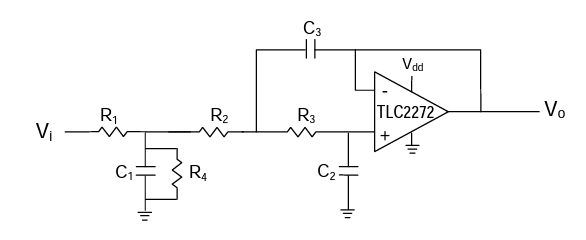
\includegraphics[width=0.5\textwidth]{./Figures/SonicSens_Filter.png}
\caption{Filter configuration from \cite{Design_SonicSens_Filter}}
\label{fig:sonicsens_filter}
\end{figure}

\begin{figure}
\centering
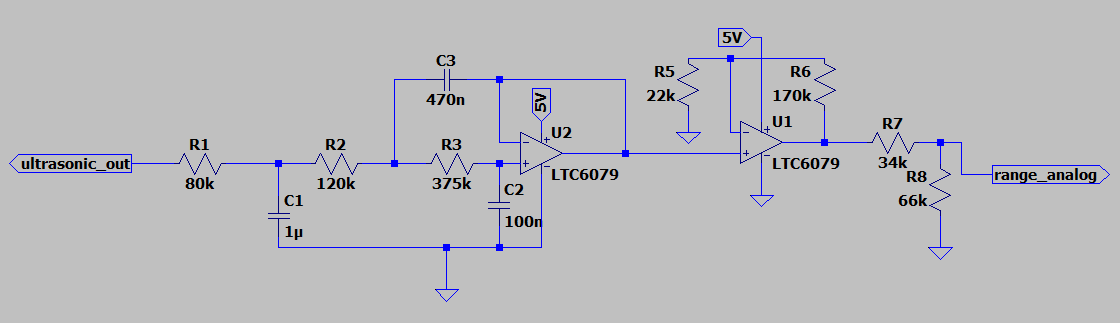
\includegraphics[width=0.5\textwidth]{./Figures/SonicSens_Diagram.png}
\caption{Filter configuration from \cite{Design_SonicSens_Filter}}
\label{fig:sonicsens_diag}
\end{figure}








\chapter{Results}\label{ch:results}
%**********************************************
\section{Current sensor} \label{sec:current_sense_results}
%**********************************************

\subsection{Simulation}

Figure \ref{fig:cursen_sim_res} shows the simulation results for the circuit shown in Figure: \ref{fig:cursen_sim_cir}. The requirement for a \SI{10}{\milli\volt} signal at \SI{1}{\kilo\hertz} to result in less than \SI{250}{\milli\volt} at the output, is shown to be met in \ref{subfig:cursen_sim_noise} where the \SI{10}{\milli\volt} signal at \SI{1}{\kilo\hertz} results in an output of $\approx$\SI{160}{\milli\volt}. Figure \ref{subfig:cursen_sim_step} shows that the circuit has a response time less than 100ms, with a response time of $\approx$\SI{30}{\milli\second}. The requirement that the amplification circuit draws less than \SI{150}{\micro\ampere} is met in Figure: \ref{subfig:cursen_sim_curdraw} where the maximum current draw is \SI{83}{\micro\ampere}.

\begin{figure}[H]
\centering
\begin{subfigure}[]{0.45\textwidth}
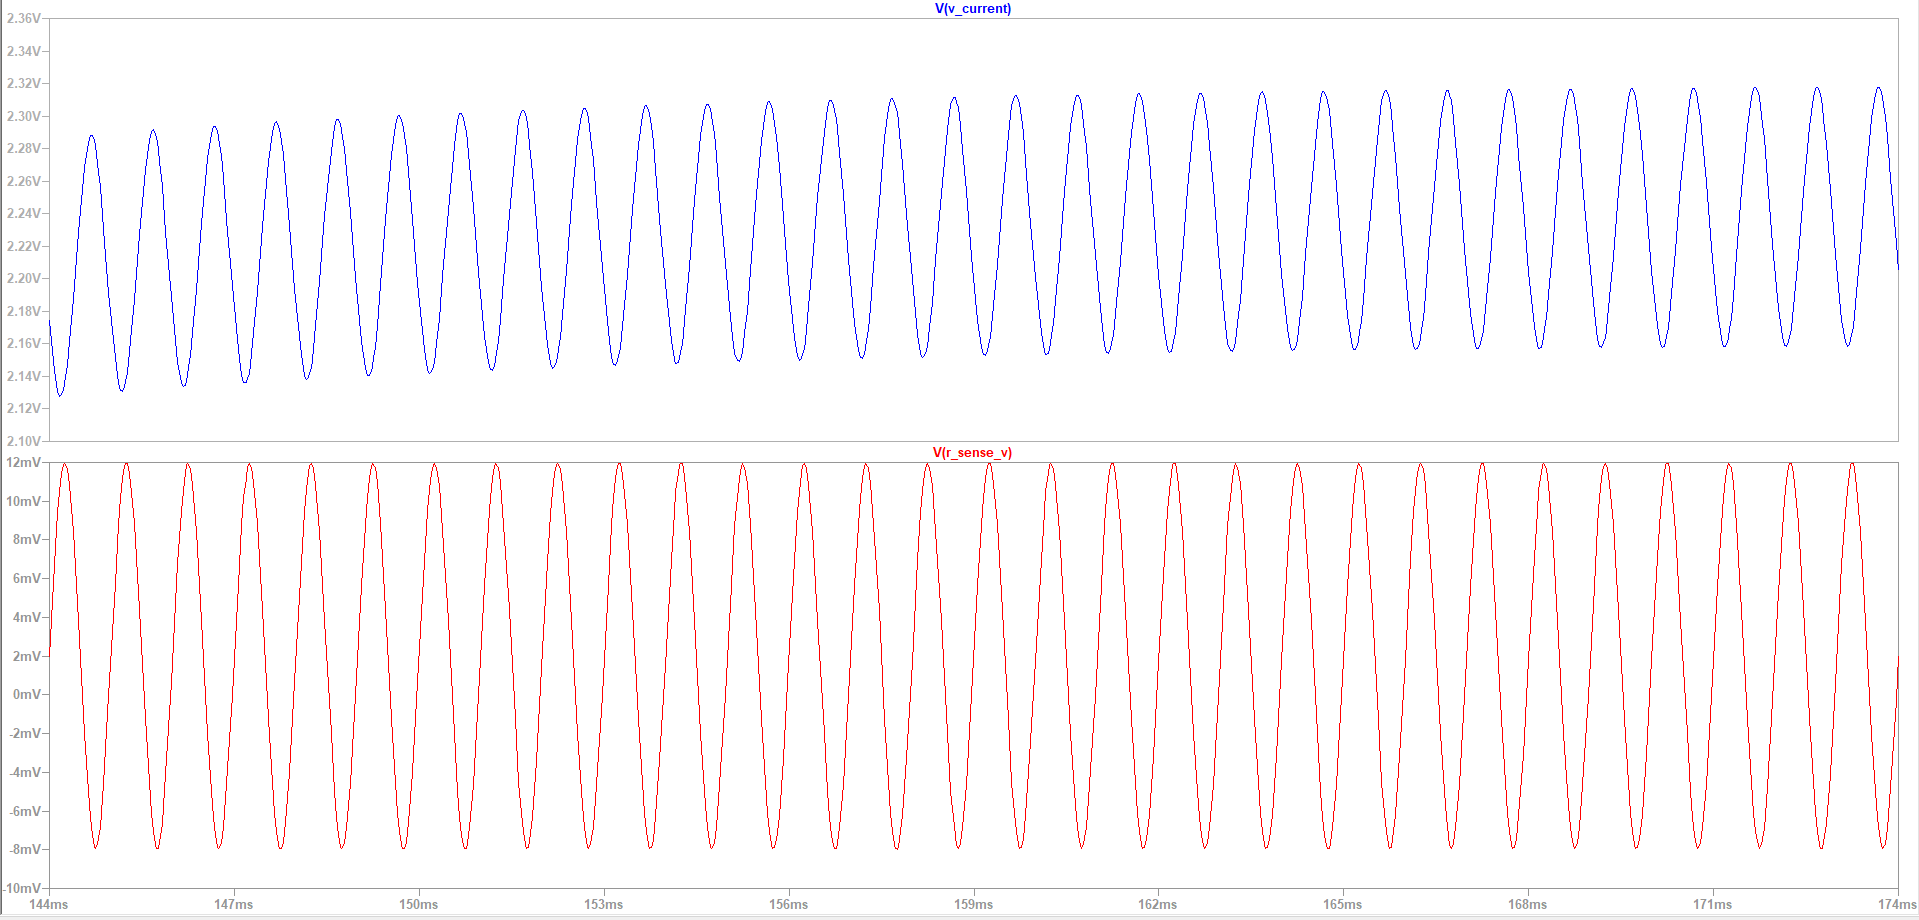
\includegraphics[width=\linewidth]{./Figures/CurSens_NoiseResp.png}
\caption{Noise input vs output of current sensing circuit.}
\label{subfig:cursen_sim_noise}	
\end{subfigure}
\hfill
\begin{subfigure}[]{0.45\textwidth}
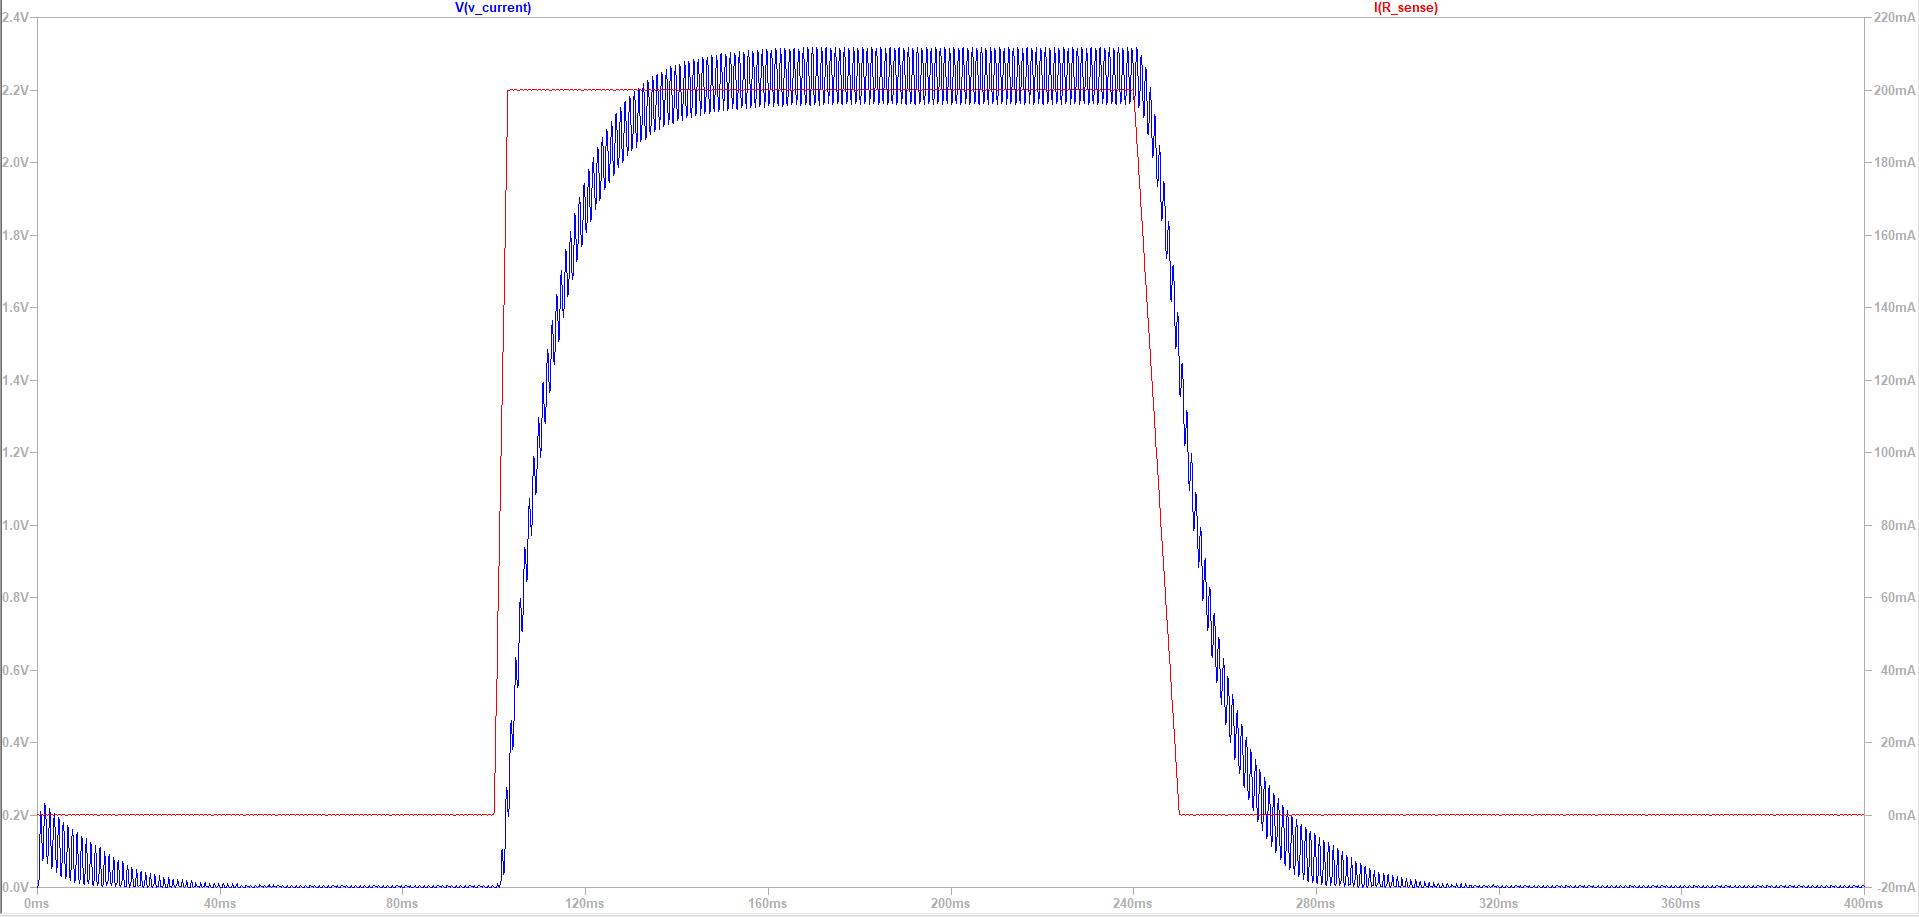
\includegraphics[width=\linewidth]{./Figures/CurSens_StepResp.png}
\caption{Step response of current sensing circuit.} 			
\label{subfig:cursen_sim_step}	
\end{subfigure}
\vspace{2pt}
\begin{subfigure}[]{0.45\textwidth}
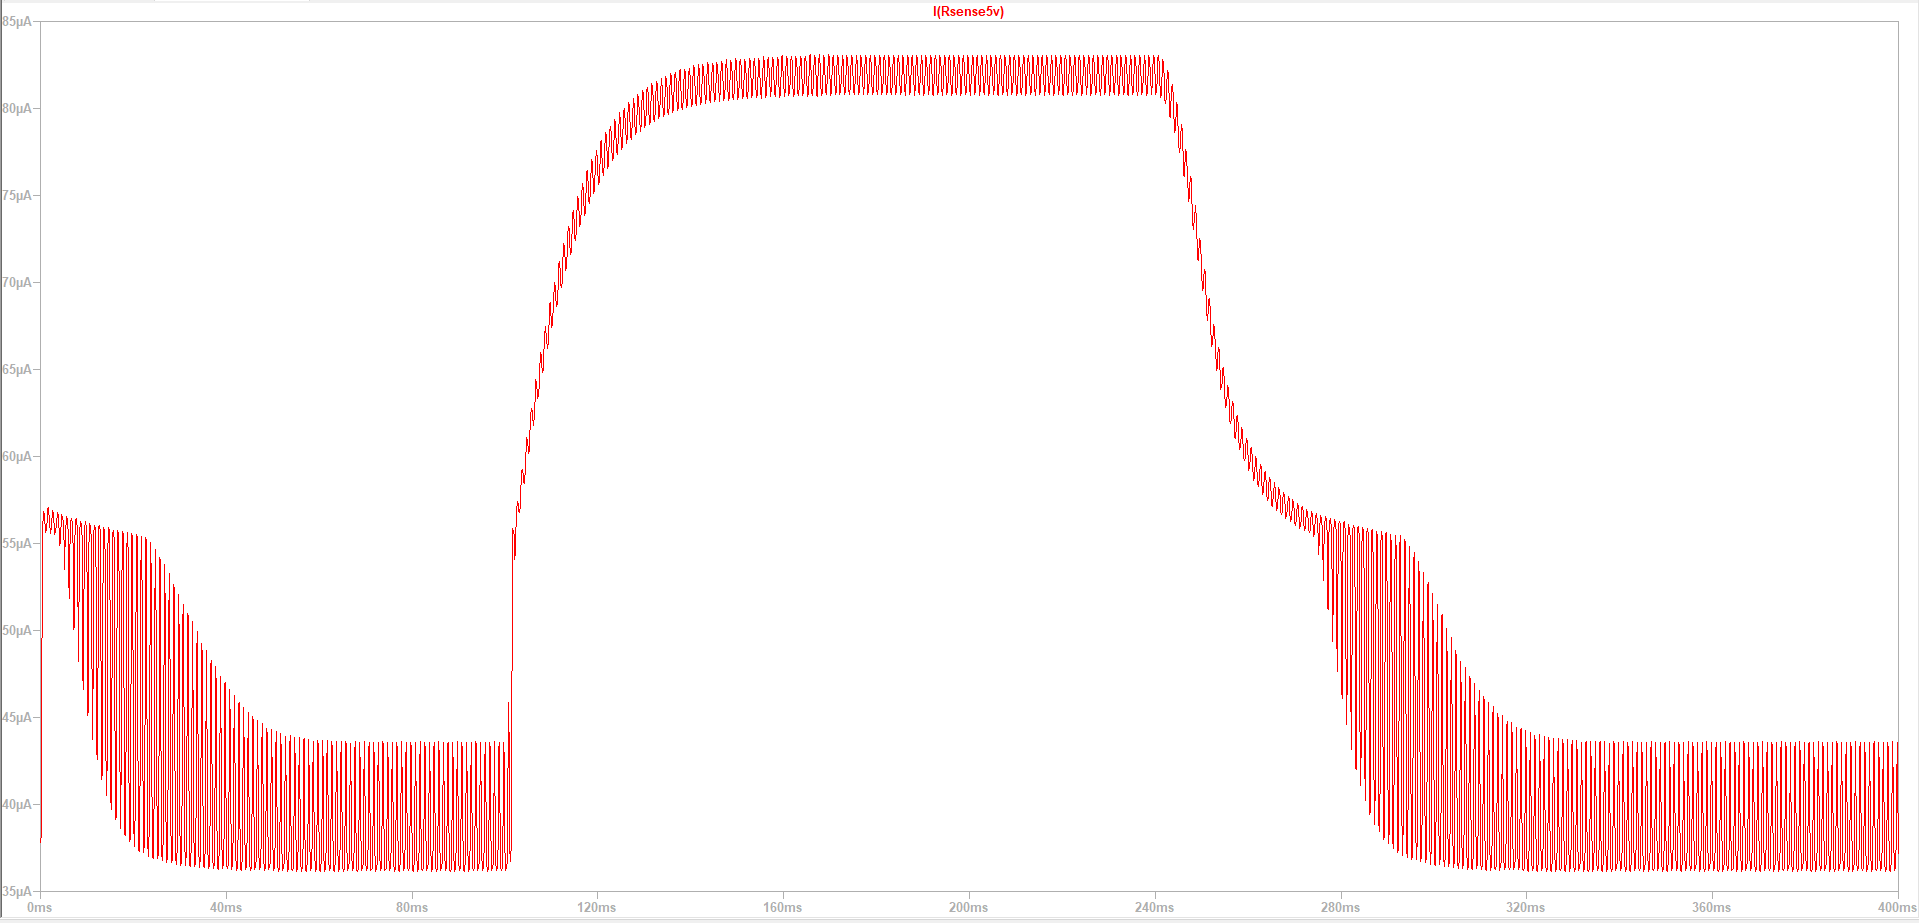
\includegraphics[width=\linewidth]{./Figures/CurSens_CurDraw.png}
\caption{Current draw of 5V supply to current sensing circuit.}
\label{subfig:cursen_sim_curdraw}	
\end{subfigure}
\caption{Current sensing circuit simulation results}
\label{fig:cursen_sim_res}
\end{figure}

\clearpage
\subsection{Practical}
As shown in Figure:\ref{fig:cursen_prac_resp} the practical results match the simulated results shown in Figure: \ref{fig:cursen_sim_res}. 

The practical response to no input (\ref{subfig:cursen_prac_noin}) shows an output of \SI{66}{\milli\volt}, this differs from the simulation output of \SI{0}{\volt} due to the non ideal nature of practical op amps and is due to the offset voltage between the input terminals.

Figure: \ref{subfig:cursen_sim_step} shows an output voltage of \SI{2.2}{\volt} to a \SI{200}{\milli\ampere} input while Figure: \ref{subfig:cursen_prac_slight} shows a \SI{1.82}{\volt} output to a  \SI{200}{\milli\ampere} input. This is due to the practical circuit having a reduced gain in comparison to the simulation. This was done to reduce the affect of the input offset voltage mentioned previously. 

Figure: \ref{subfig:cursen_prac_stall} shows the output clips sat \SI{3.28}{\volt} which is very close to the theoretical \SI{3.3}{\volt}. 

Figure: \ref{subfig:cursen_prac_noise} shows a lesser response to noise than the simulation, this is due to the noise input to the practical circuit is different to the simulated noise and at a higher frequency so the low pass filter attenuates it more heavily.

The measure response time in Figure: \ref{subfig:cursen_prac_step} is \SI{24}{\milli\second} which is very close to the response time measured in the simulation of \SI{30}{\milli\second}.


\begin{figure}[H]
\centering
\begin{subfigure}[]{0.3\textwidth}
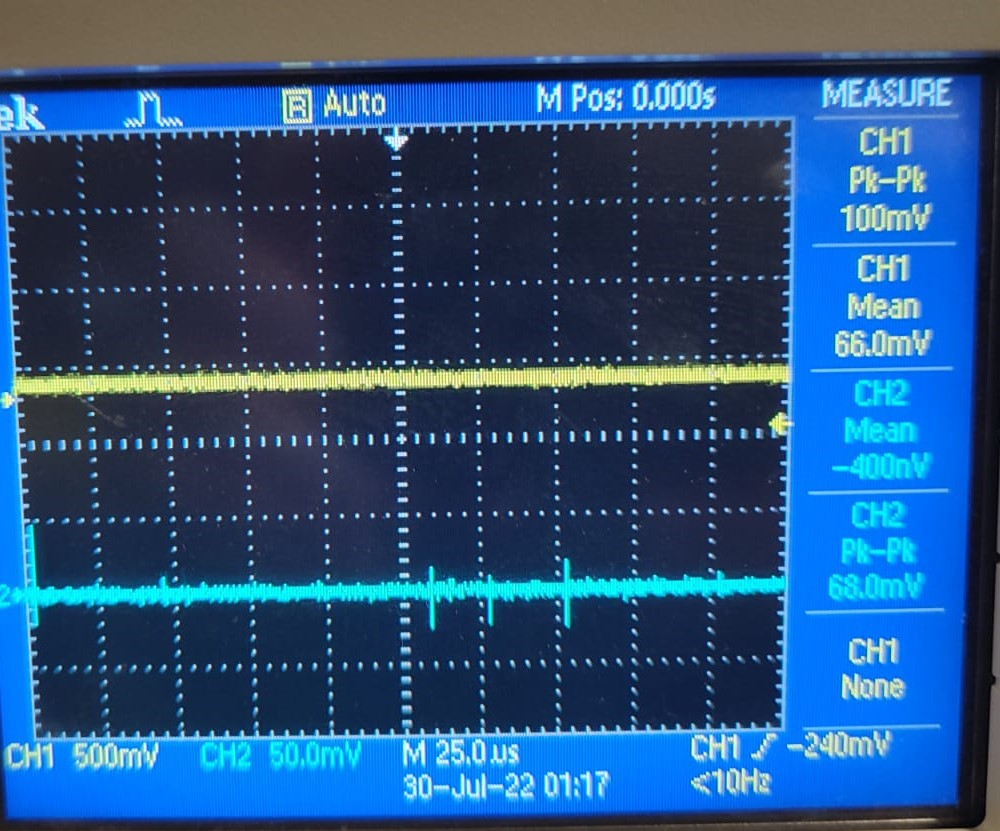
\includegraphics[width=\linewidth]{./Figures/CurSens_Prac_0input.jpeg}
\caption{Circuit response to no input.}
\label{subfig:cursen_prac_noin}	
\end{subfigure}
\hfill
\begin{subfigure}[]{0.3\textwidth}
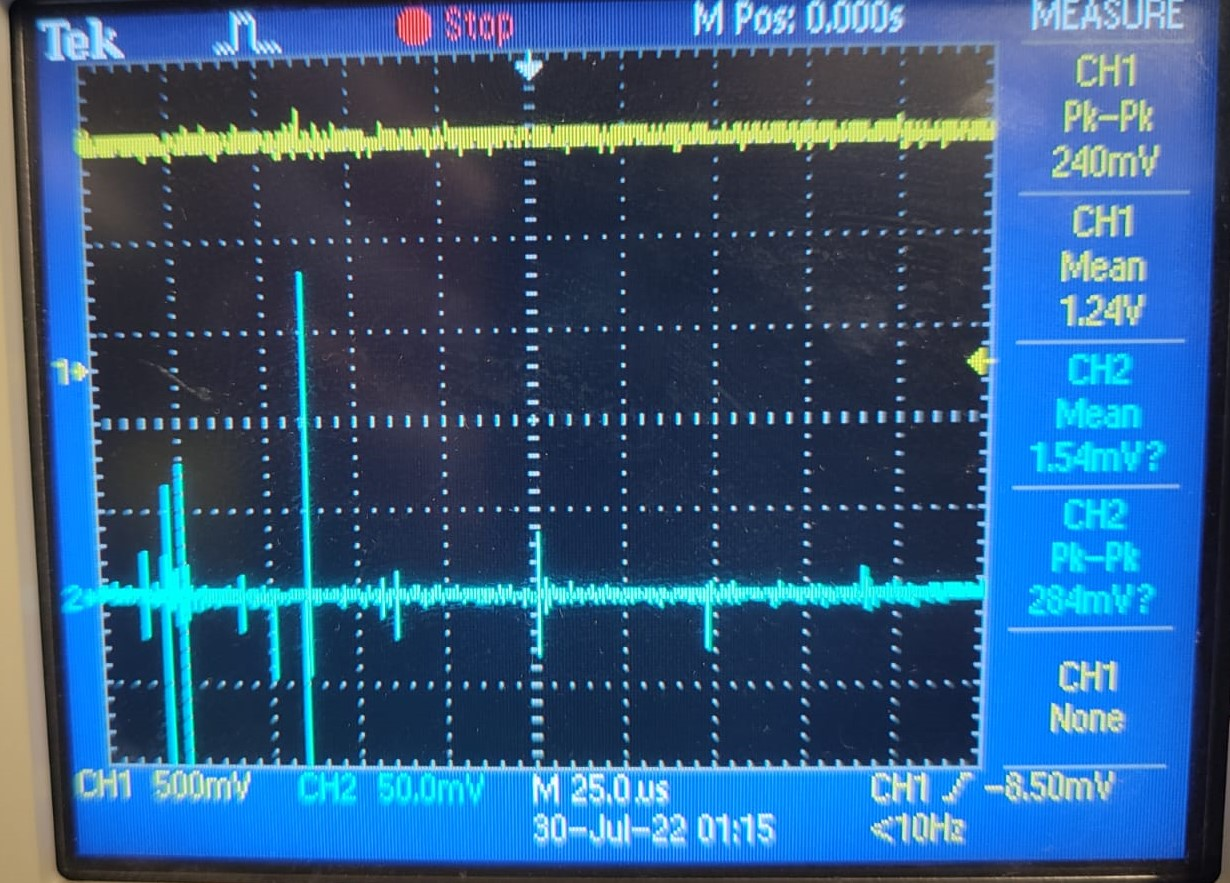
\includegraphics[width=\linewidth]{./Figures/CurSens_Prac_Free.jpeg}
\caption{Circuit response to free running motor.} 			
\label{subfig:cursen_prac_free}	
\end{subfigure}
\hfill
\begin{subfigure}[]{0.3\textwidth}
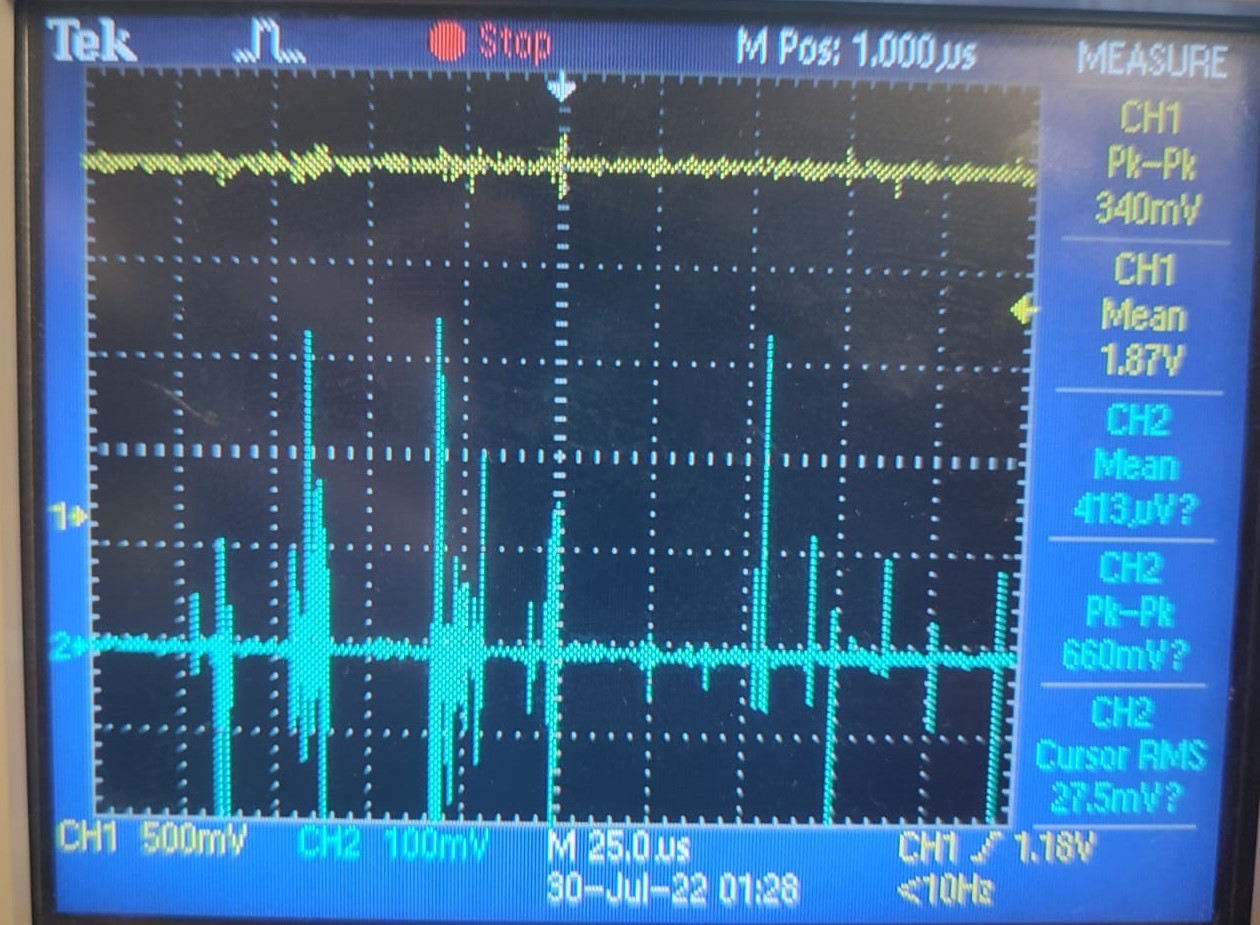
\includegraphics[width=\linewidth]{./Figures/CurSens_Prac_Slight.jpeg}
\caption{Circuit response to slight restriction on the motor.}
\label{subfig:cursen_prac_slight}	
\end{subfigure}
\vfill
\begin{subfigure}[]{0.3\textwidth}
\includegraphics[width=\linewidth]{./Figures/CurSens_Prac_Stall.jpeg}
\caption{Circuit response to motor stall.}
\label{subfig:cursen_prac_stall}	
\end{subfigure}
\hfill
\begin{subfigure}[]{0.3\textwidth}
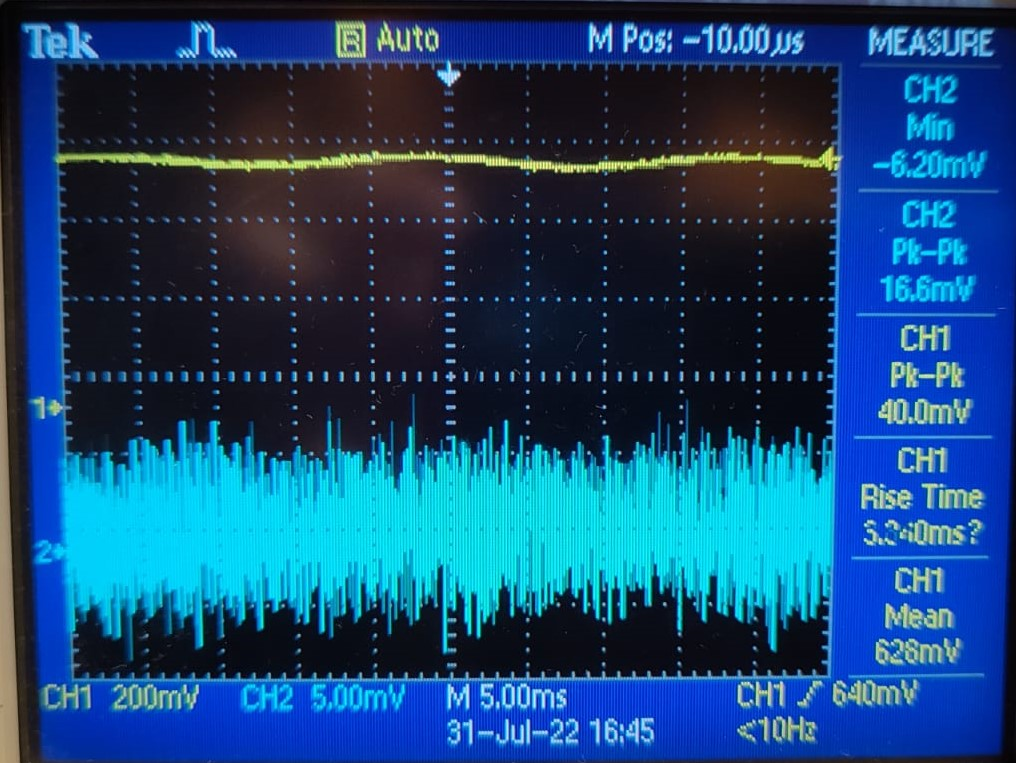
\includegraphics[width=\linewidth]{./Figures/CurSens_Prac_Noise.jpeg}
\caption{Circuit response to noise.}
\label{subfig:cursen_prac_noise}	
\end{subfigure}
\hfill
\begin{subfigure}[]{0.3\textwidth}
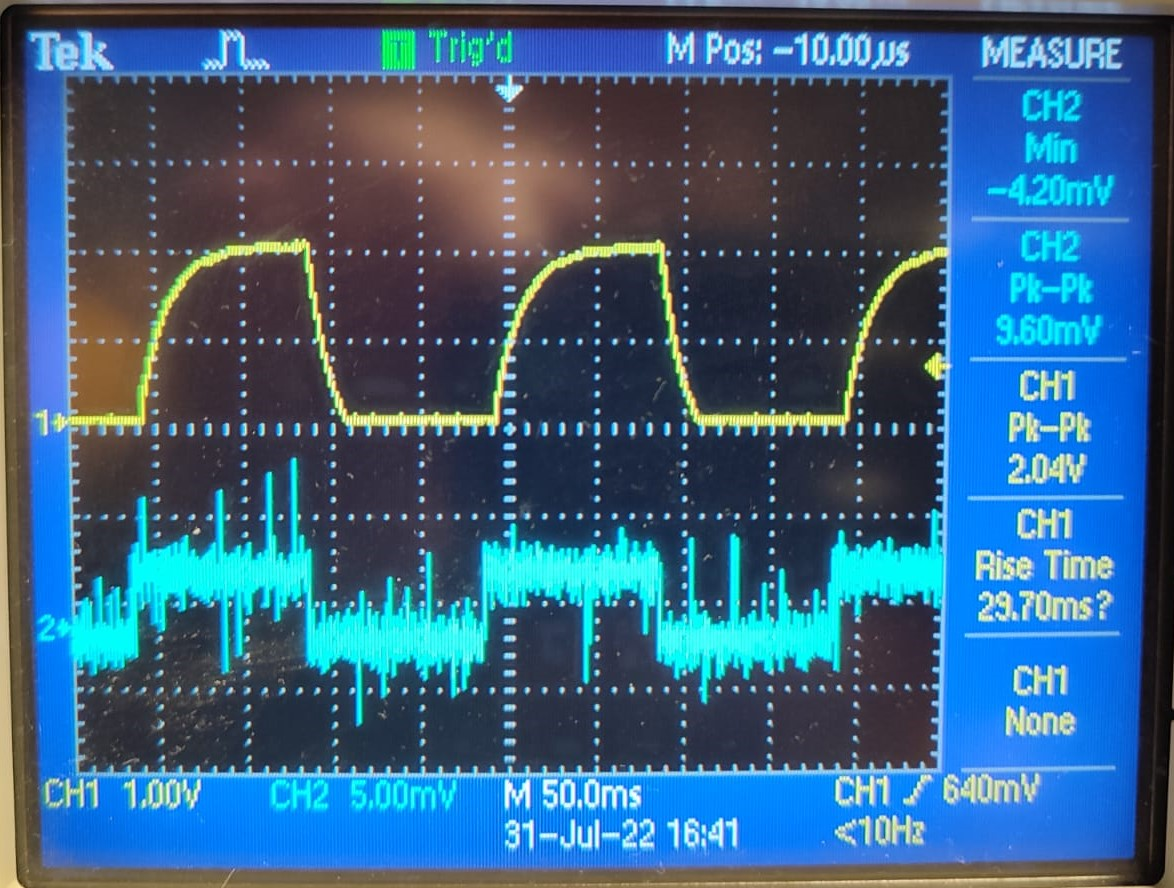
\includegraphics[width=\linewidth]{./Figures/CurSens_Prac_Step.jpeg}
\caption{Circuit response to step input.} 			
\label{subfig:cursen_prac_step}	
\end{subfigure}
\caption{Circuit response to different input conditions}
\label{fig:cursen_prac_resp}
\end{figure}

\newpage

\subsection{Circuit}
\begin{figure}[H]
\centering
\includegraphics[width = 0.9\textwidth]{./Figures/Cursens_Cir_Card.jpeg}
\caption{Labelled circuit and student card.}
\label{fig:cursen_cir_card}
\end{figure}

\clearpage
\section{Ultrasonic range sensor}
\subsection{Simulation}

Figure: \ref{fig:sonicsen_sim_step} shows the circuit response to a step input change from the maximum 10\% duty cycle to a 0.5\% duty cycle. As shown in the figure the circuit outputs > \SI{3}{\volt} for a maximum input and < \SI{0.3}{\volt} for the minimum input. The figure also demonstrates the circuits compliance to the noise and response time requirements with noise levels of \SI{58}{\milli\volt}pk-pk and a response time of \SI{386}{\milli\second}.

Figure: \ref{fig:sonicsen_sim_cur} shows that throughout circuit operation current draw is < \SI{170}{\micro\ampere}.

\begin{figure}[H]
\centering
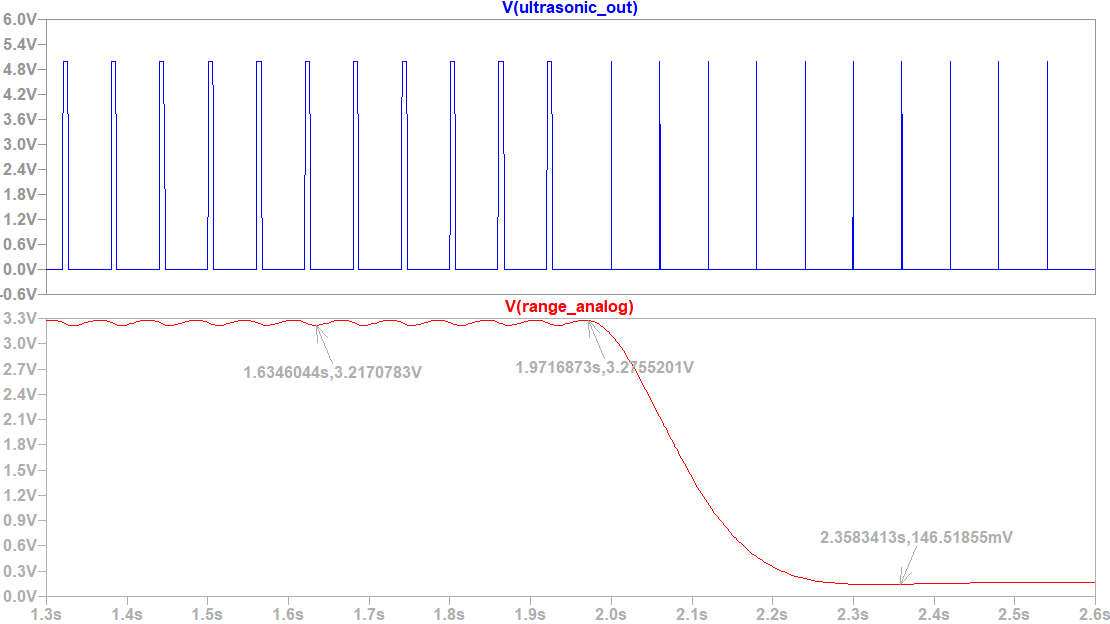
\includegraphics[width = 0.5\textwidth]{./Figures/SonicSens_RangeStep.png}
\caption{Circuit response to a full range step from 10\% to 0.5\% duty cycle}
\label{fig:sonicsen_sim_step}
\end{figure}

\begin{figure}[H]
\centering
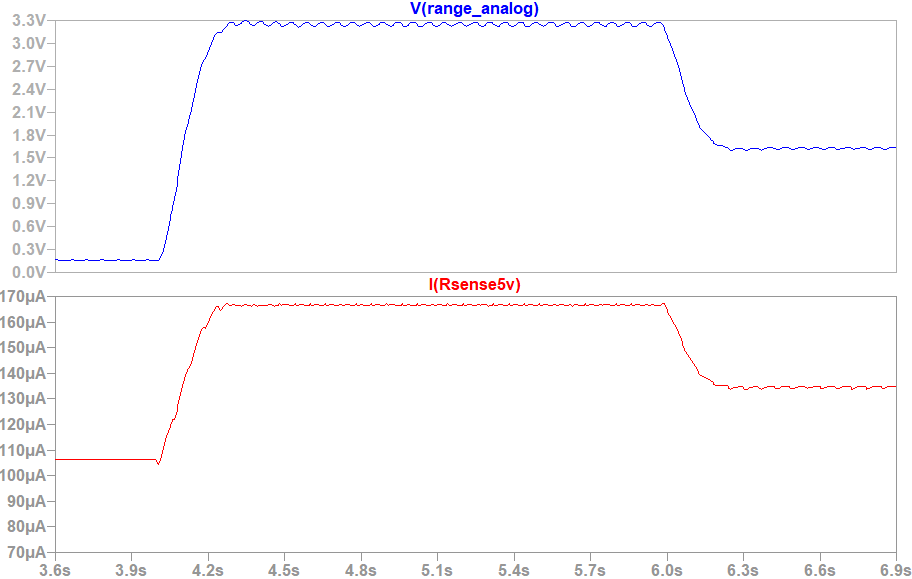
\includegraphics[width = 0.5\textwidth]{./Figures/SonicSens_CurDraw.png}
\caption{Current draw vs circuit output}
\label{fig:sonicsen_sim_cur}
\end{figure}

\clearpage
\subsection{Practical}

Figure: \ref{fig:sonicsen_sim_step} shows the output response to a step change from \SI{1}{\meter} to \SI{5}{\centi\meter} back to \SI{1}{\meter}. The figure also shows the compliance to the requirements with the \SI{1}{\meter} measurement having an output of \SI{3.24}{\volt} and an output of \SI{200}{\milli\volt} at \SI{5}{\centi\meter}. The figure also shows a compliance with the rise time of \SI{258}{\milli\second}.

Figure: \ref{subfig:sonicsen_prac_ripple} shows that the output ripple voltage is less than \SI{70}{\milli\volt}pk-pk at \SI{1}{\meter} when the ripple voltage will be at its worst.

Figure: \ref{subfig:sonicsen_prac_range} shows the circuit response to a gradual change in the input across the full range from close to far.

\begin{figure}[H]
\centering
\begin{subfigure}[]{0.45\textwidth}
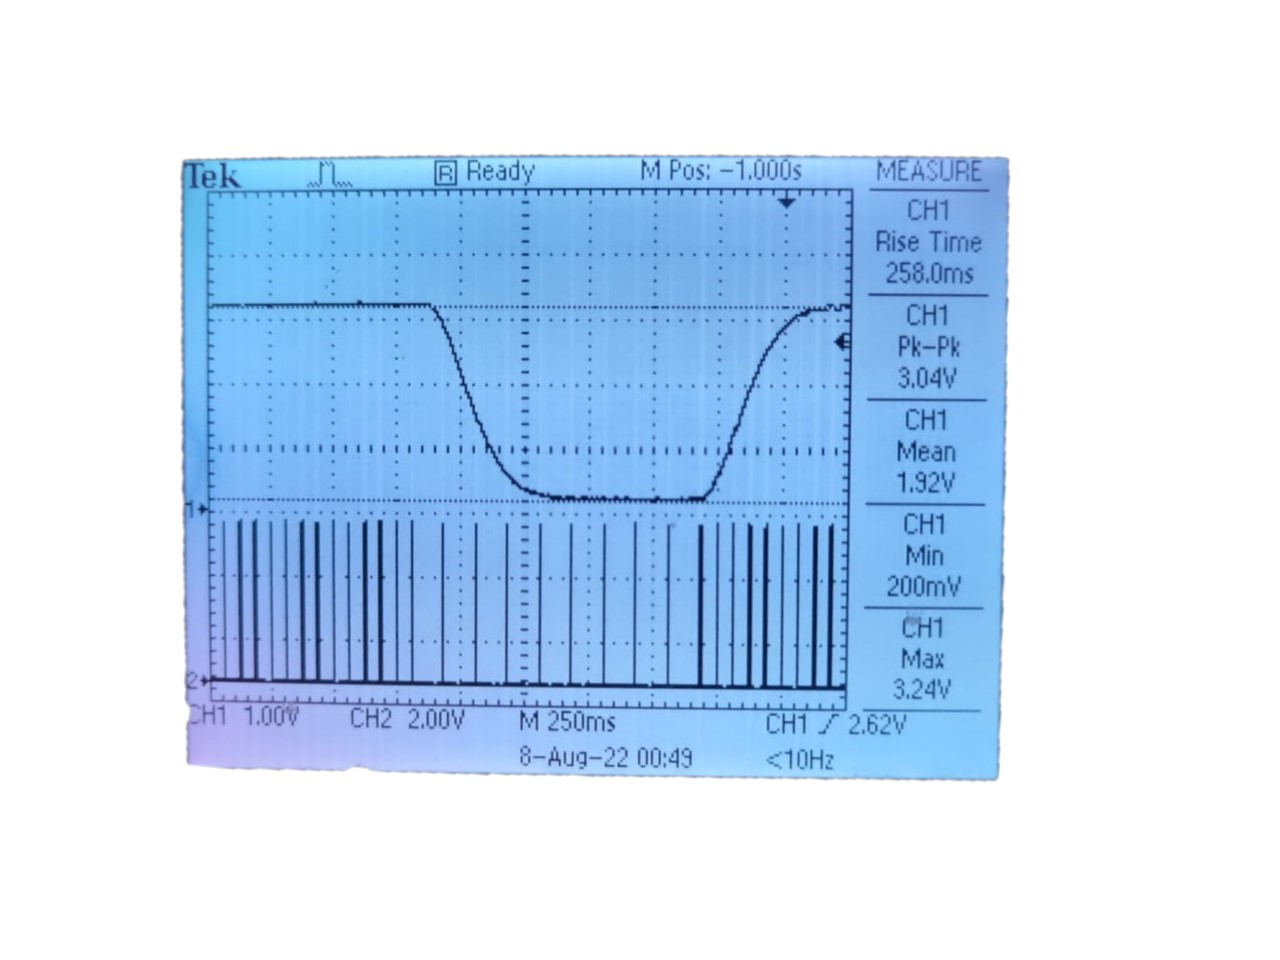
\includegraphics[width=\linewidth]{./Figures/SonicSens_Prac_Step.jpeg}
\caption{Circuit response a step input.}
\label{subfig:sonicsen_prac_step}	
\end{subfigure}
\hfill
\begin{subfigure}[]{0.45\textwidth}
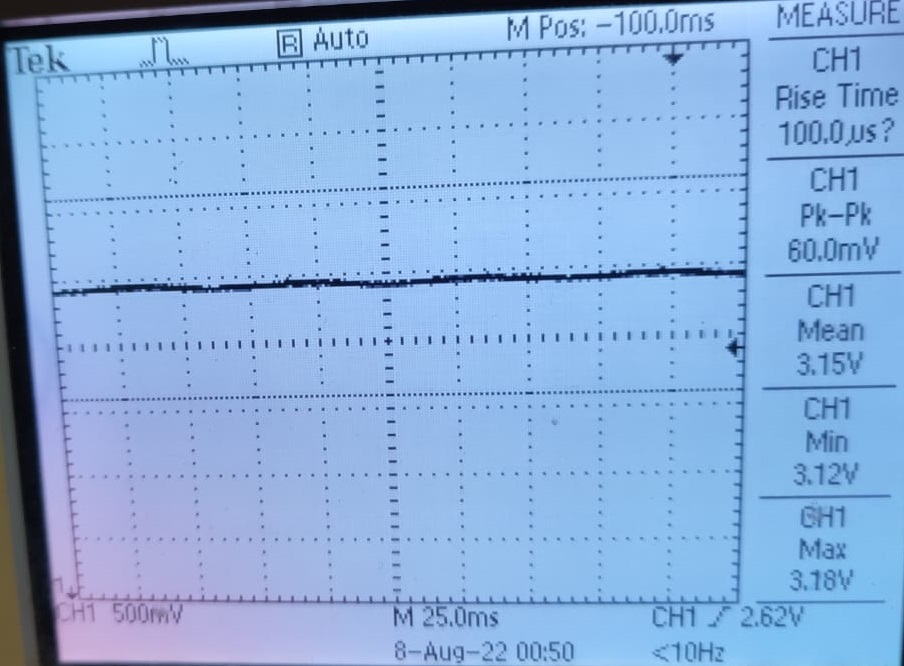
\includegraphics[width=\linewidth]{./Figures/SonicSens_Prac_Ripple.jpeg}
\caption{Circuit ripple voltage at 1m.} 			
\label{subfig:sonicsen_prac_ripple}	
\end{subfigure}
\vfill
\begin{subfigure}[]{0.45\textwidth}
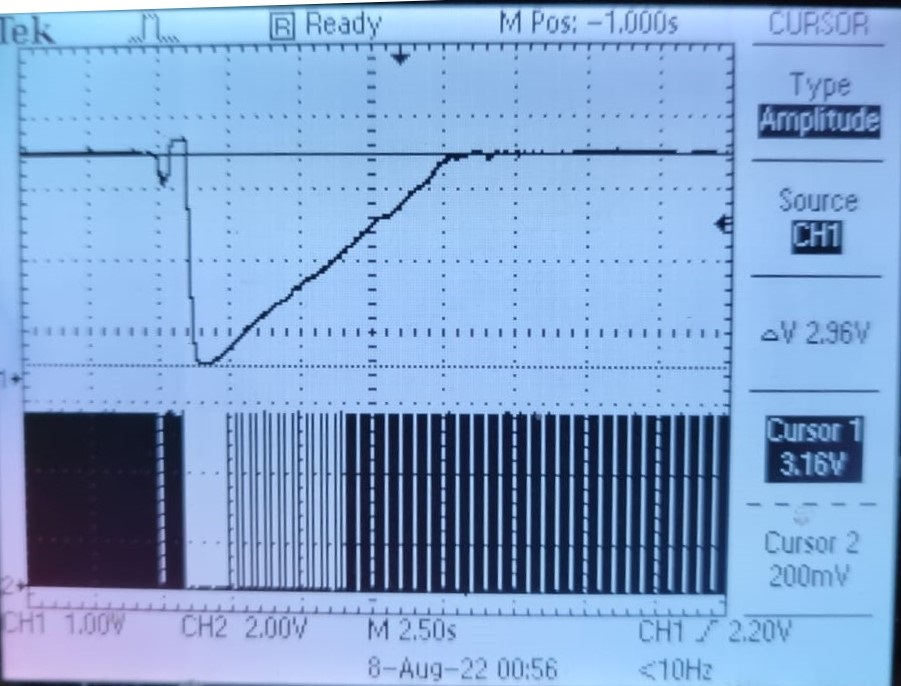
\includegraphics[width=\linewidth]{./Figures/SonicSens_Prac_Range.jpeg}
\caption{Circuit response to smooth change in range measurement.}
\label{subfig:sonicsen_prac_range}	
\end{subfigure}
\caption{Ultrasonic sensor filter circuit responses.}
\label{fig:sonicsen_prac}
\end{figure}

\newpage
\subsection{Circuit}
\begin{figure}[H]
\centering
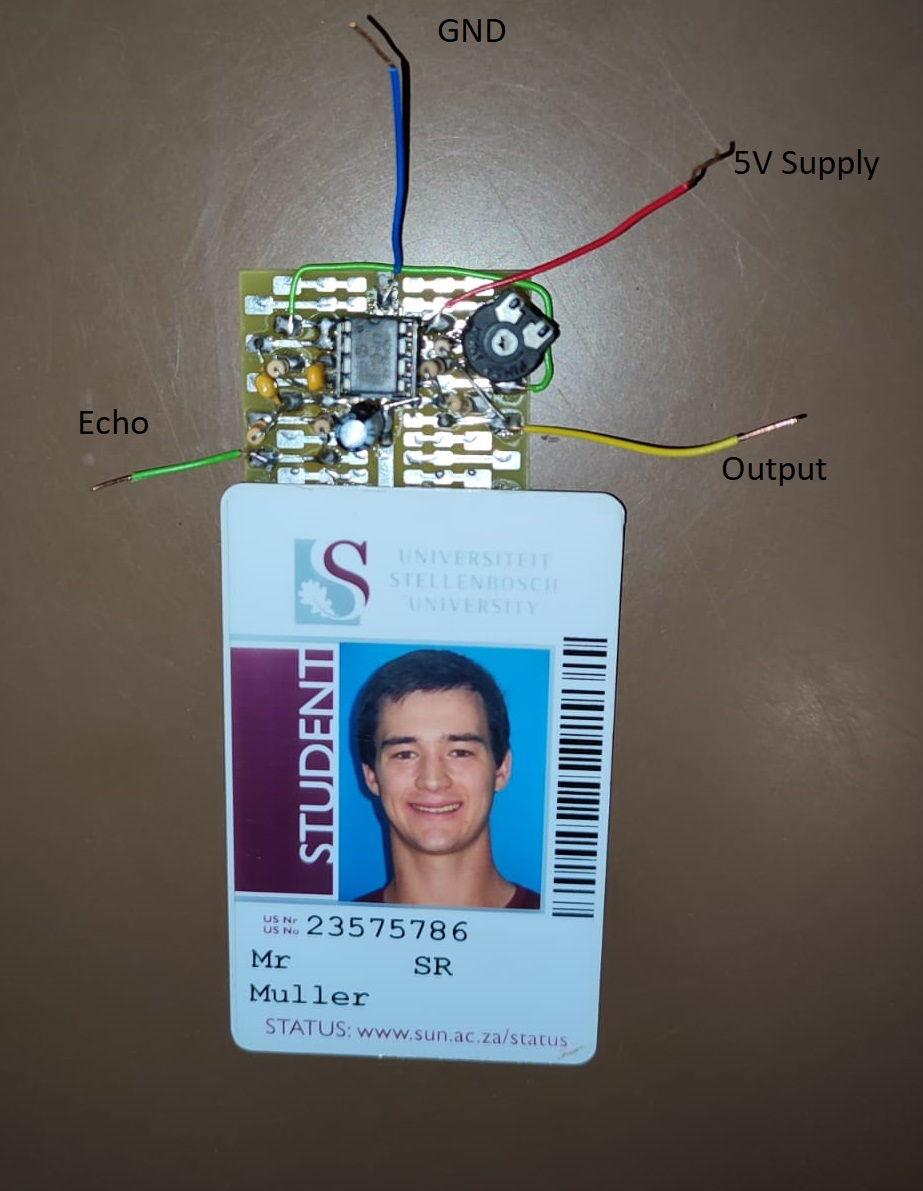
\includegraphics[width = 0.9\textwidth]{./Figures/SonicSens_Cir_Card.jpeg}
\caption{Labelled circuit and student card.}
\label{fig:sonicsen_cir_card}
\end{figure}

\clearpage
\section{Digital to analogue converter}
\subsection{Simulation}
Figure: \ref{fig:dac_sim_out} shows the simulation output vs the given input and that the simulated results match the requirements. Figure: \ref{fig:dac_sim_cur} shows that the current draw for the simulated circuit is at acceptable levels.  
\begin{figure}[H]
\centering
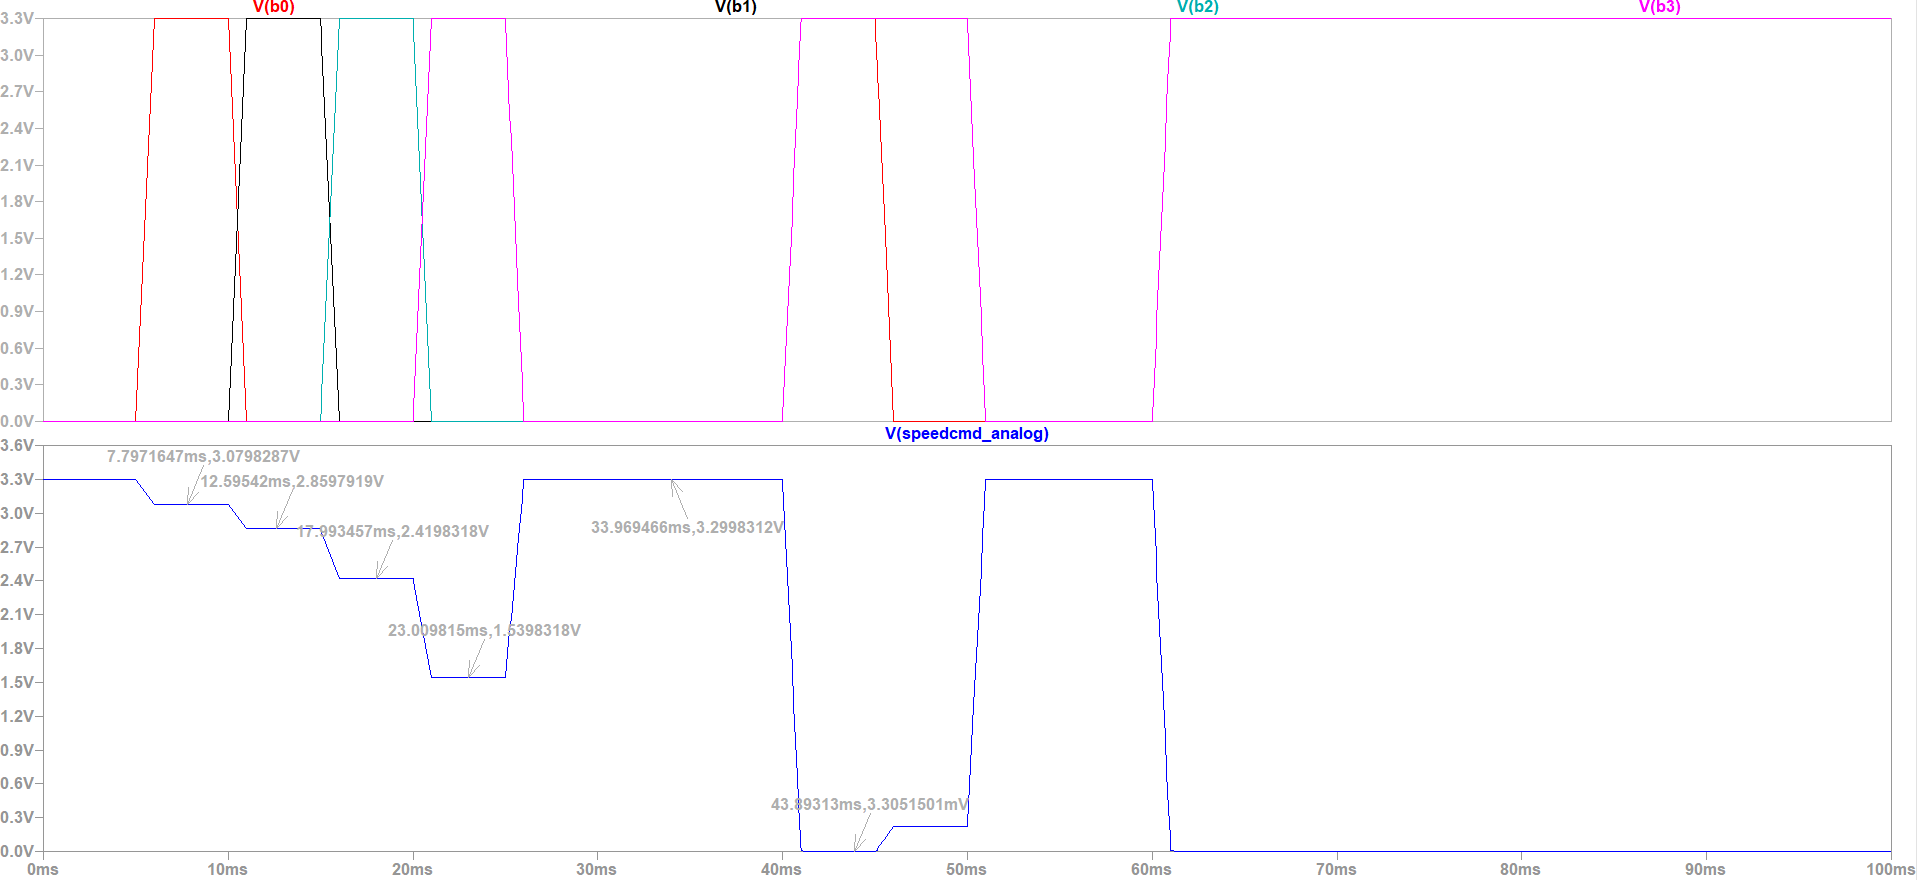
\includegraphics[width = 0.7\textwidth]{./Figures/DAC_Sim_Out.png}
\caption{Output vs input of DAC.}
\label{fig:dac_sim_out}
\end{figure}

\begin{figure}[H]
\centering
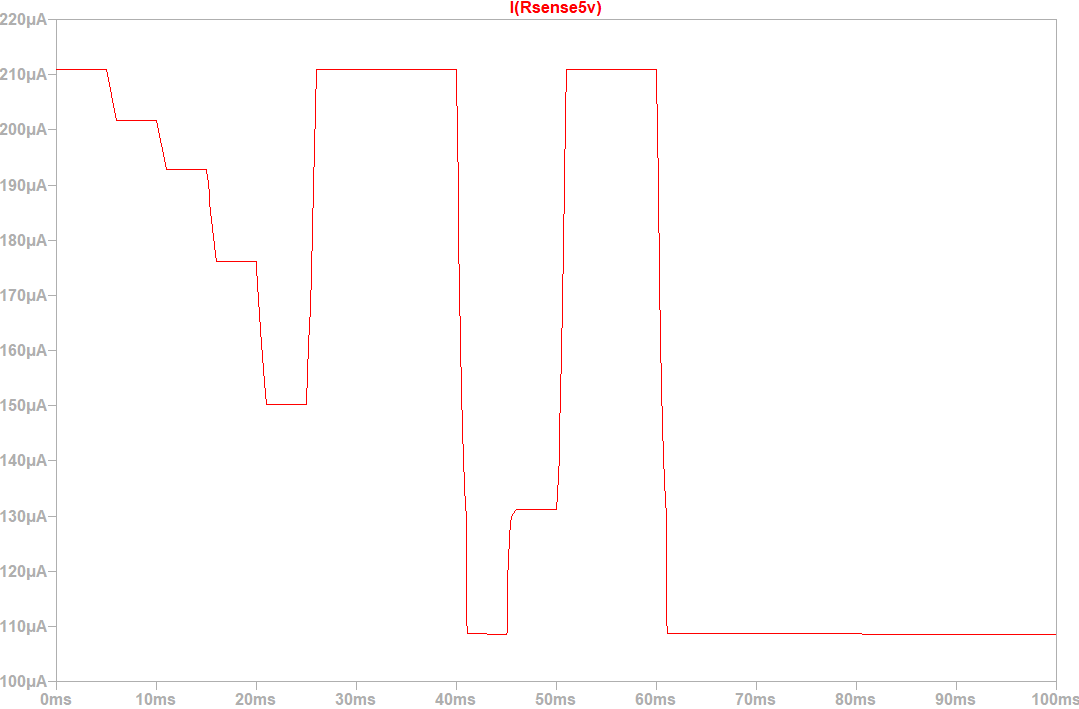
\includegraphics[width = 0.7\textwidth]{./Figures/DAC_Sim_Cur.png}
\caption{Current draw of the DAC circuit}
\label{fig:dac_sim_cur}
\end{figure}

\clearpage
\subsection{Practical}
Figure: \ref{fig:dac_prac} shows the DAC response to different inputs. Figure: \ref{subfig:dac_prac_0000} shows that the circuit complies with the requirement to have an output larger than \SI{3}{\volt} for an input of 0. Figure: \ref{subfig:dac_prac_1111} shows the circuit complies with the requirement that the output is less than \SI{0.5}{\volt}.
\begin{figure}[H]
\centering
\begin{subfigure}[]{0.3\textwidth}
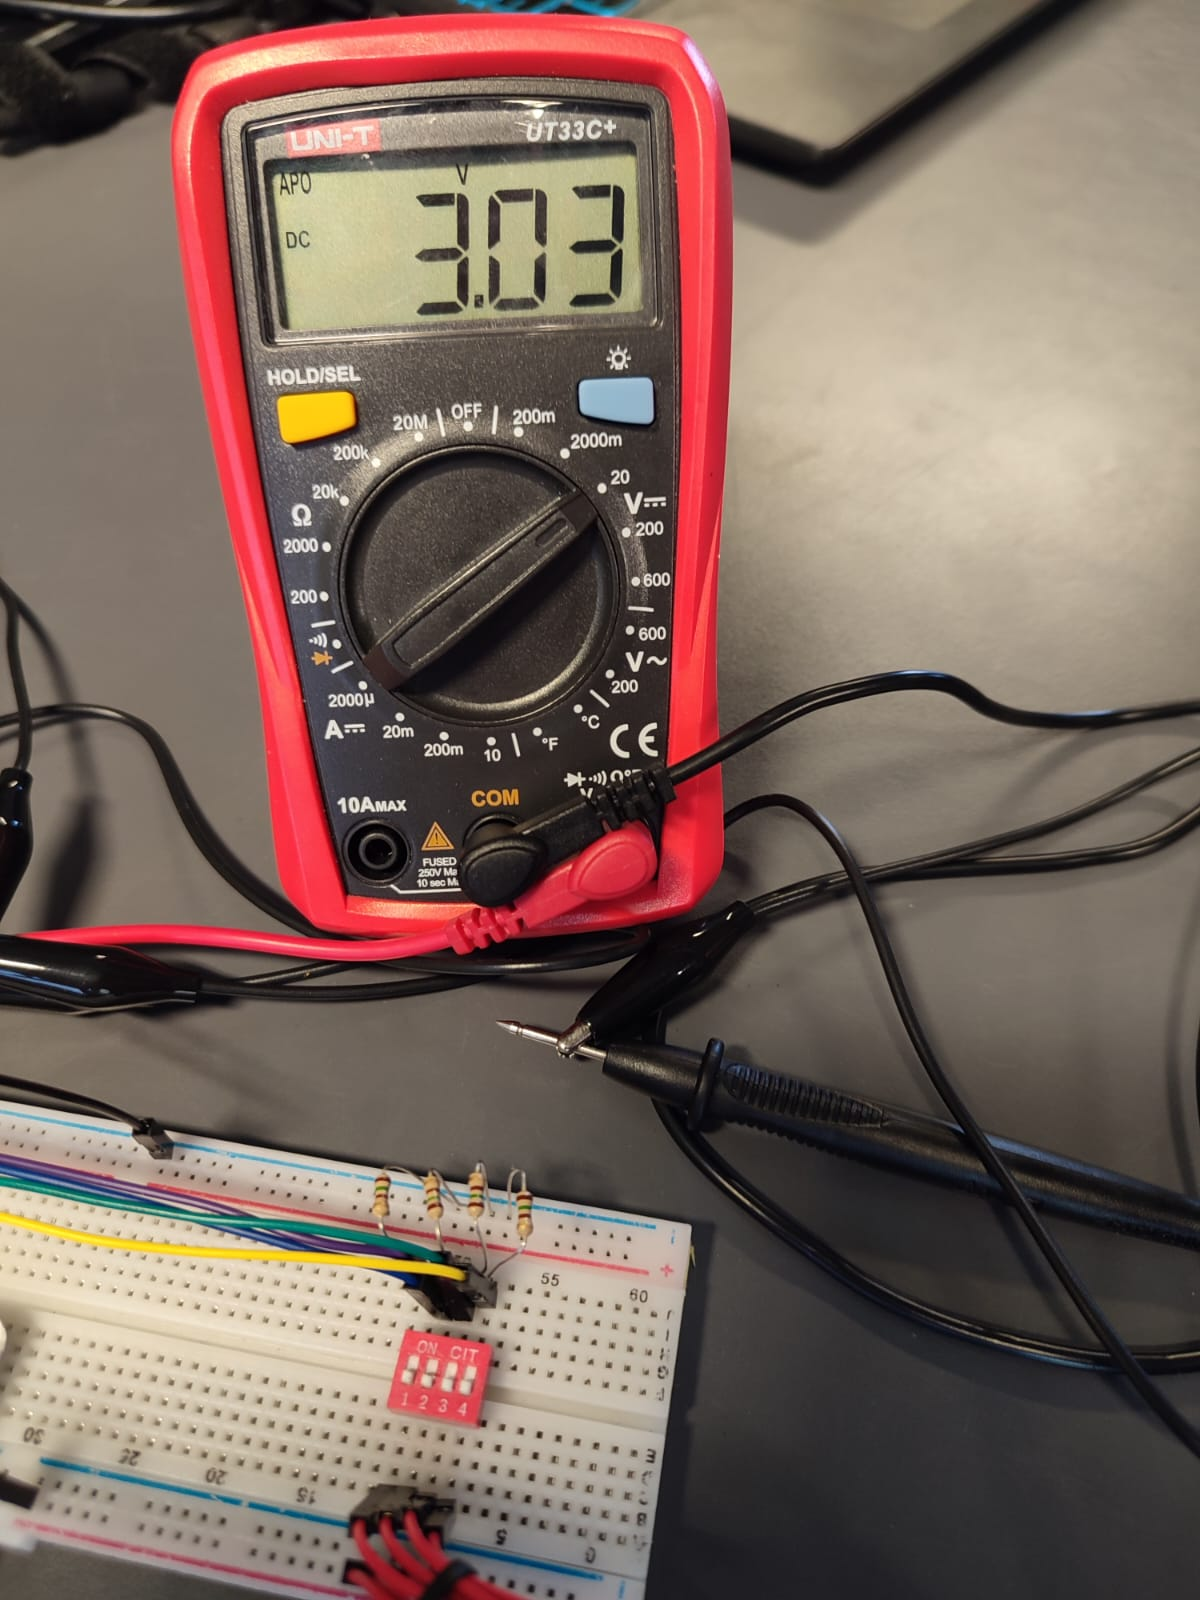
\includegraphics[width=\linewidth]{./Figures/DAC_Prac_0000.jpeg}
\caption{DAC output for 0000 input.}
\label{subfig:dac_prac_0000}	
\end{subfigure}
\hfill
\begin{subfigure}[]{0.3\textwidth}
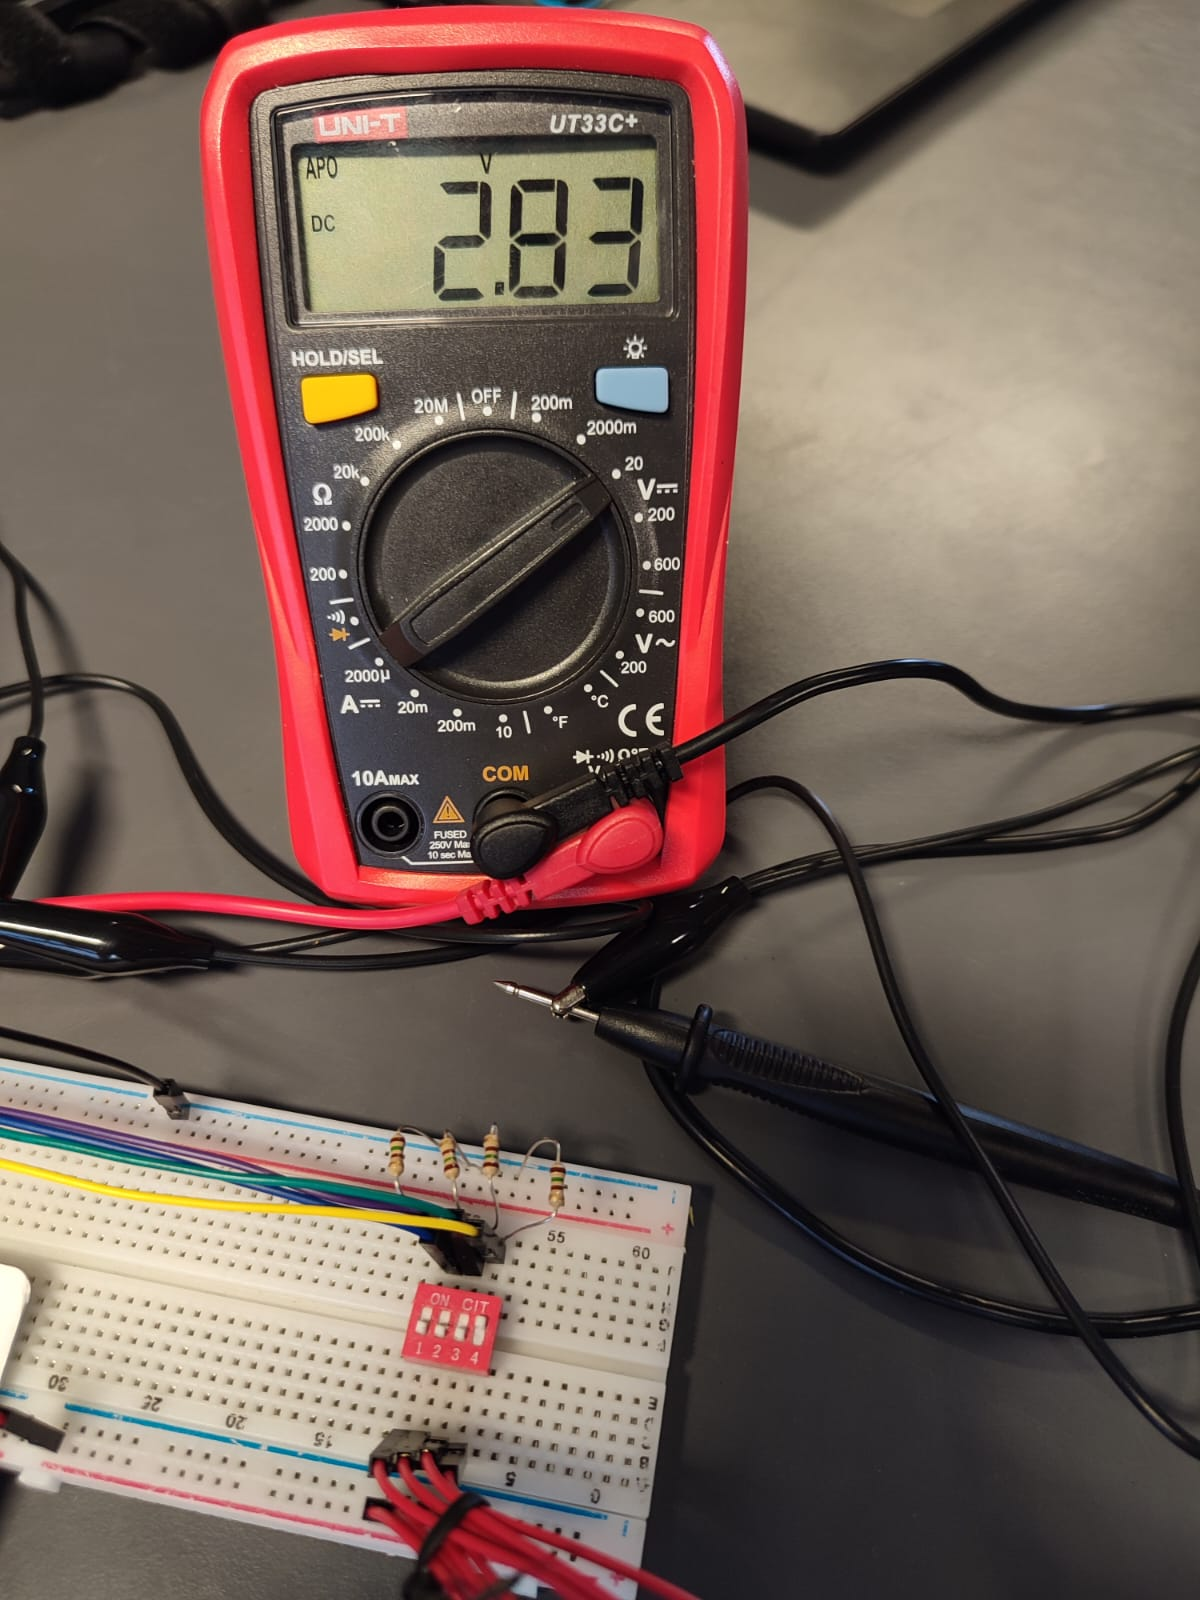
\includegraphics[width=\linewidth]{./Figures/DAC_Prac_0001.jpeg}
\caption{DAC output for 0001 input.} 			
\label{subfig:dac_prac_0001}	
\end{subfigure}
\hfill
\begin{subfigure}[]{0.3\textwidth}
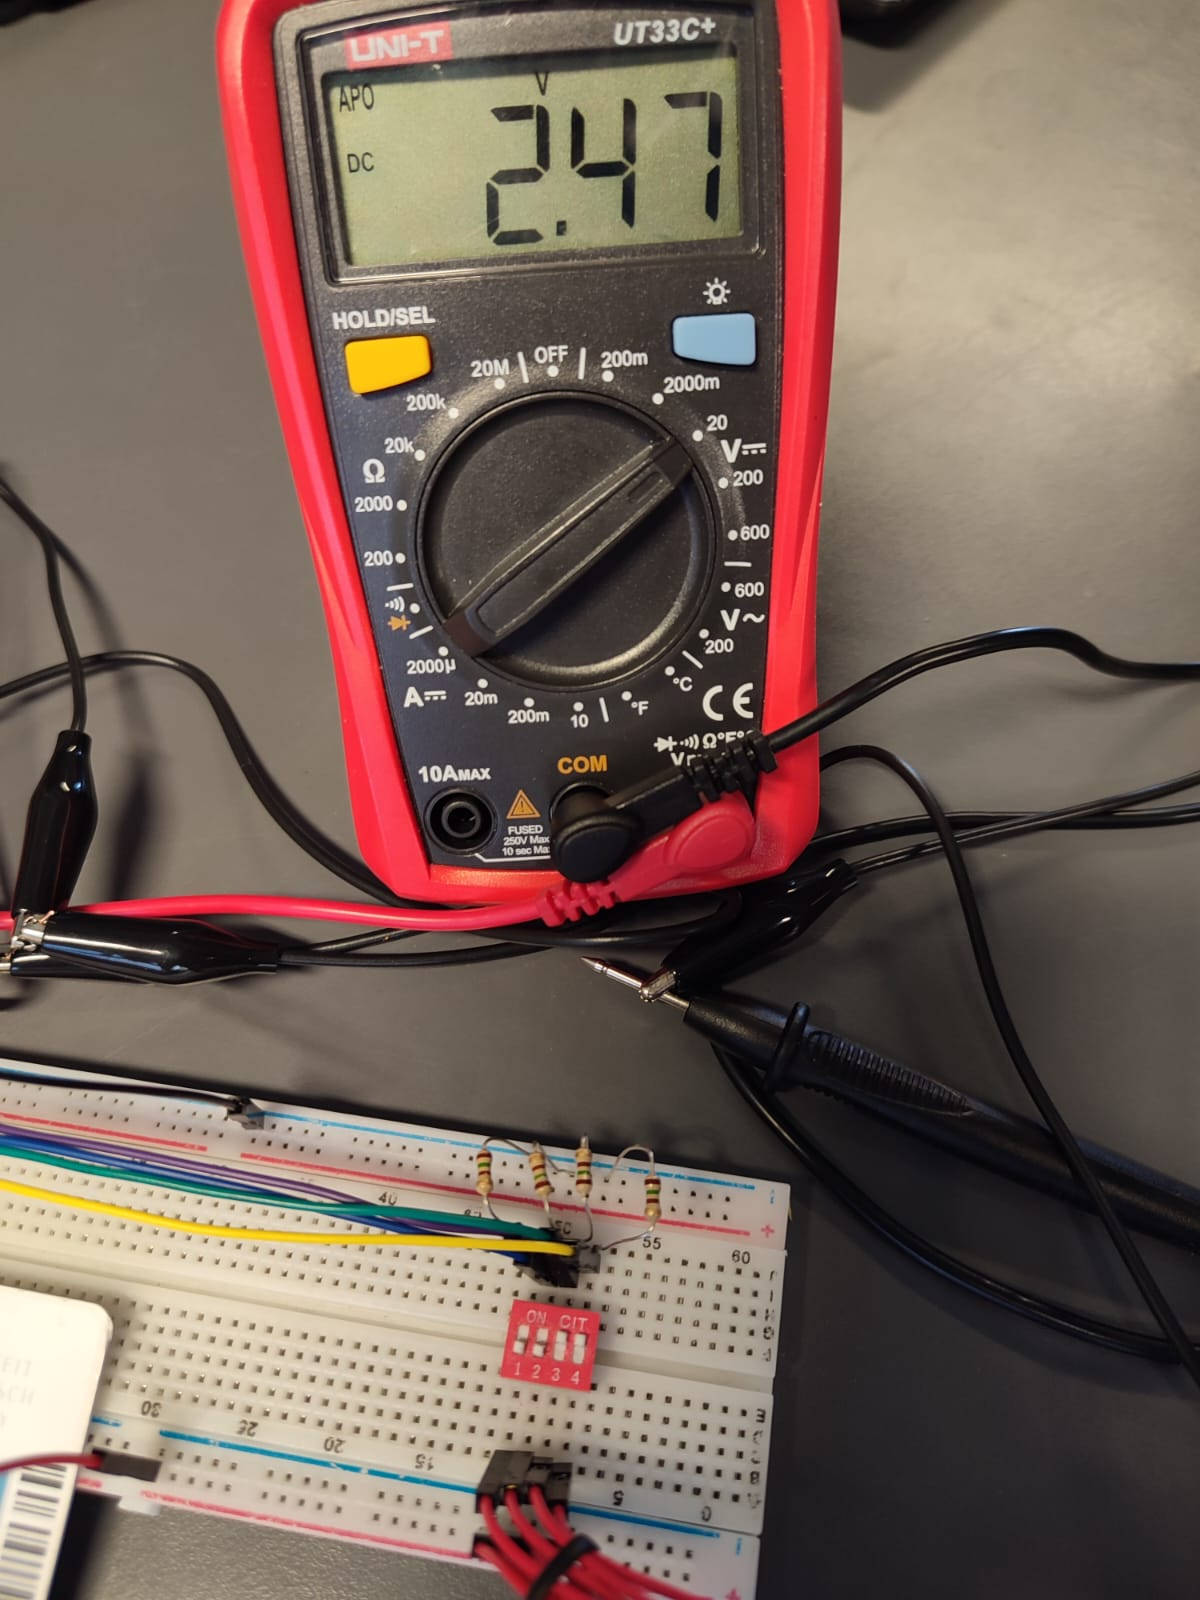
\includegraphics[width=\linewidth]{./Figures/DAC_Prac_0011.jpeg}
\caption{DAC output for 0011 input.} 			
\label{subfig:dac_prac_0011}	
\end{subfigure}
\vfill
\begin{subfigure}[]{0.3\textwidth}
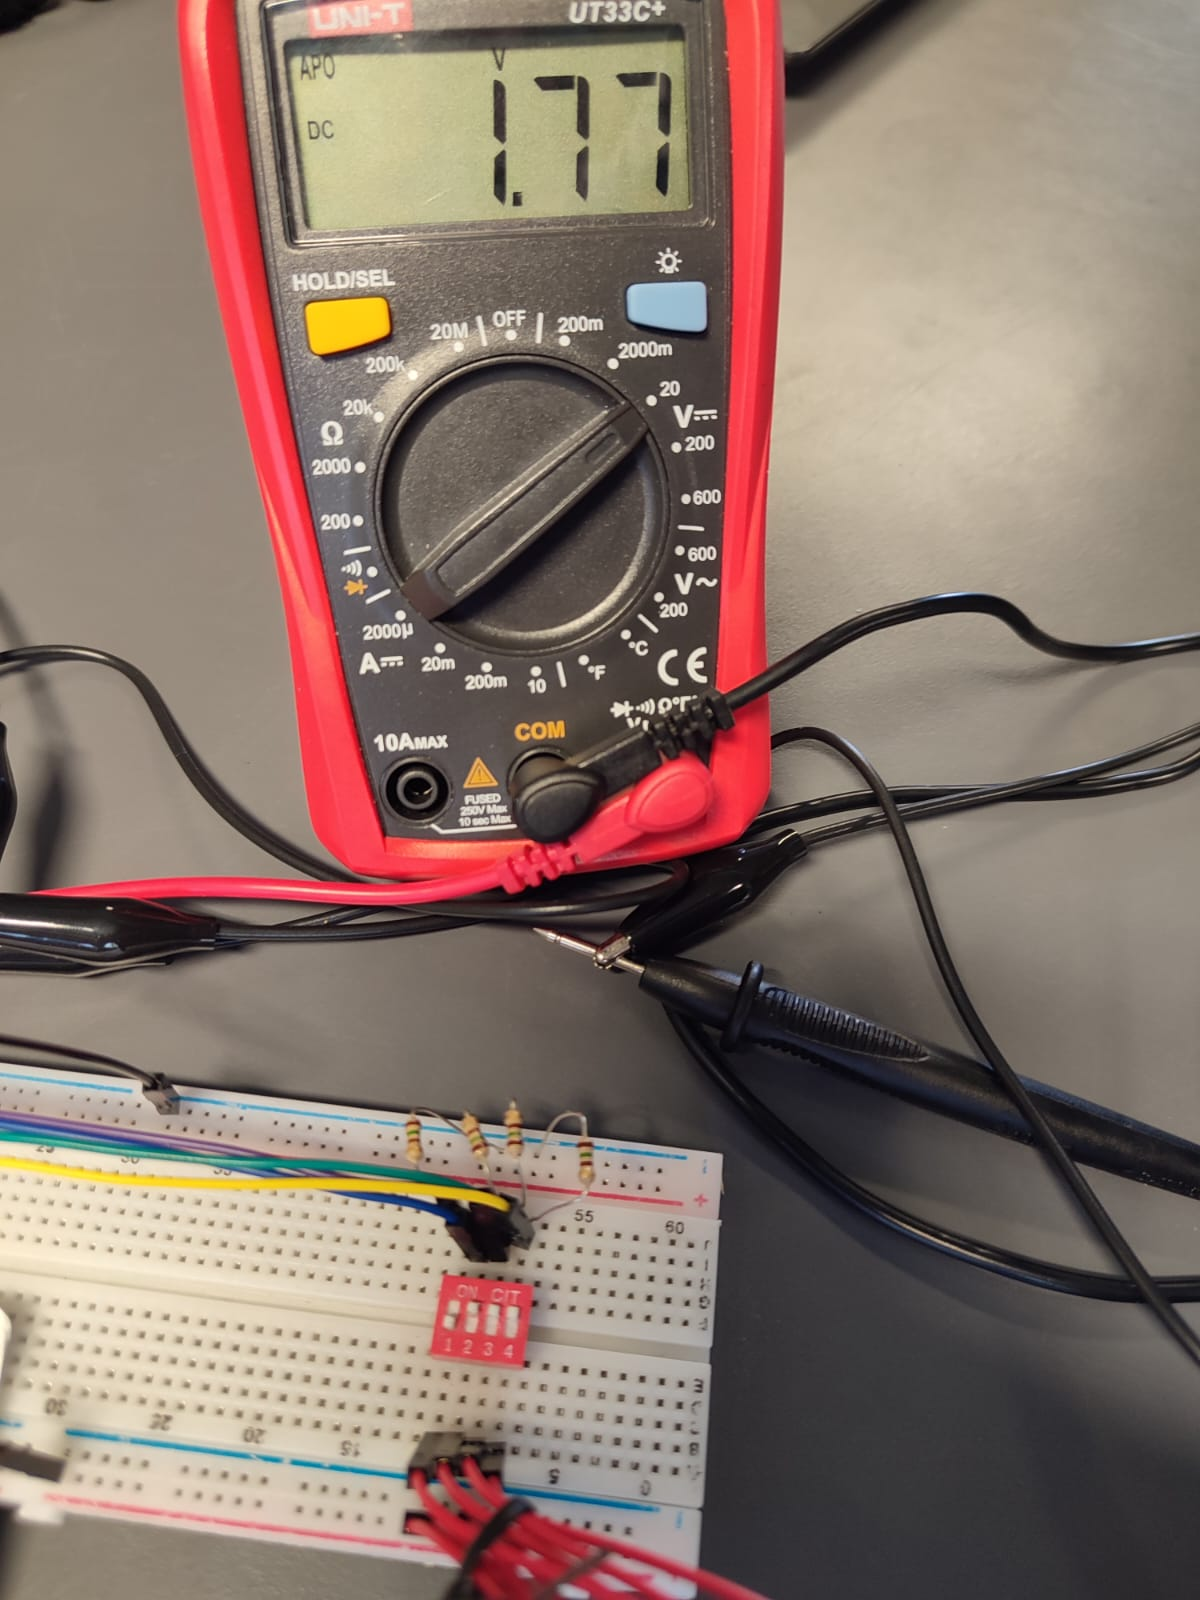
\includegraphics[width=\linewidth]{./Figures/DAC_Prac_0111.jpeg}
\caption{DAC output for 0111 input.}
\label{subfig:dac_prac_0111}	
\end{subfigure}
\hfill
\begin{subfigure}[]{0.3\textwidth}
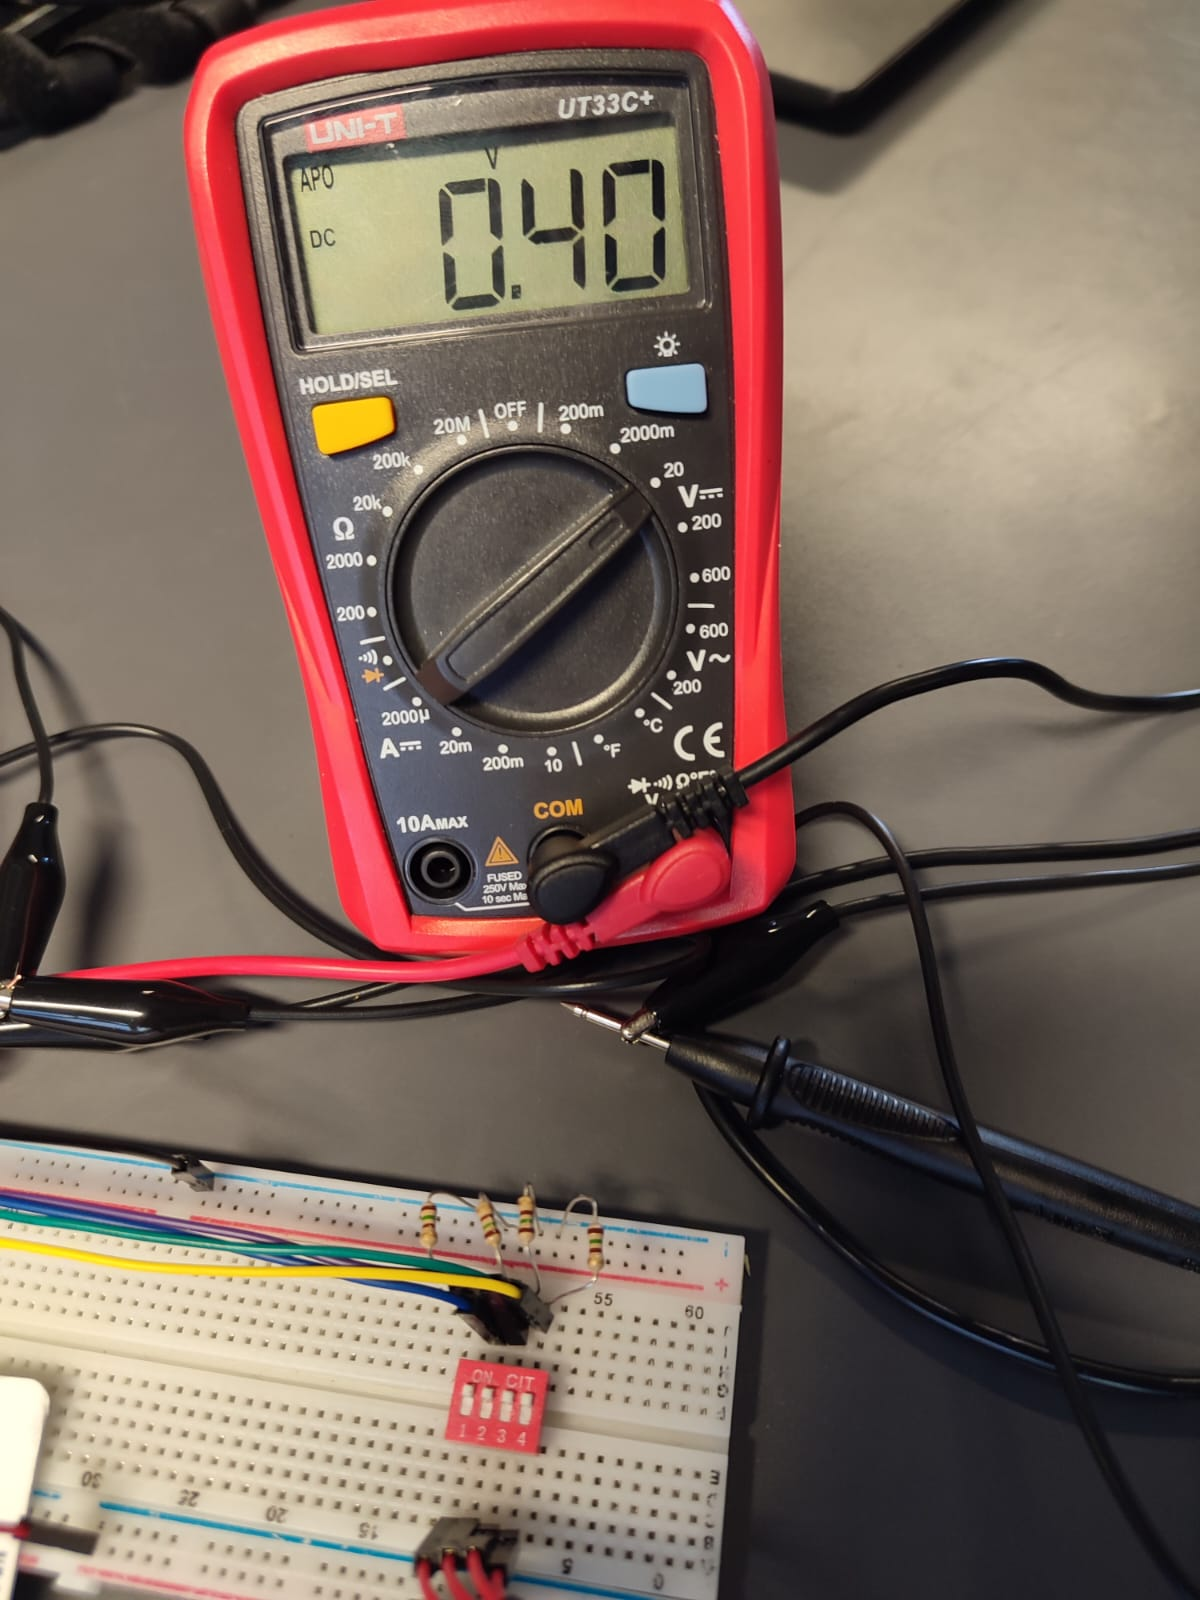
\includegraphics[width=\linewidth]{./Figures/DAC_Prac_1111.jpeg}
\caption{DAC output for 1111 input.}
\label{subfig:dac_prac_1111}
\end{subfigure}
\hfill
\begin{subfigure}[]{0.3\textwidth}
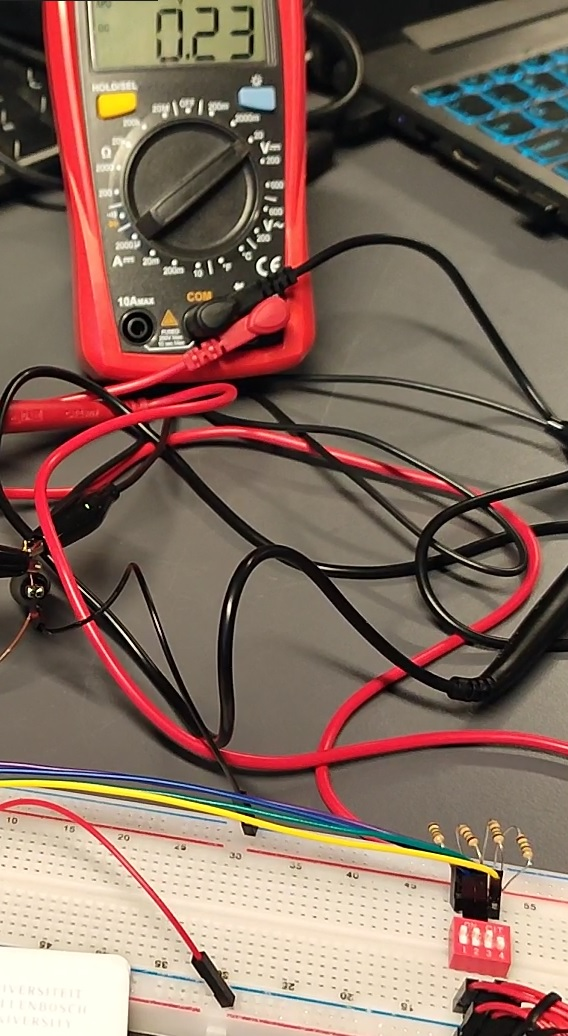
\includegraphics[width=\linewidth]{./Figures/DAC_Prac_1110.jpeg}
\caption{DAC output for 1110 input.} 			
\label{subfig:dac_prac_1110}	
\end{subfigure}
\caption{DAC output for different inputs.}
\label{fig:dac_prac}
\end{figure}

\clearpage
\subsection{Circuit}
\begin{figure}[H]
\centering
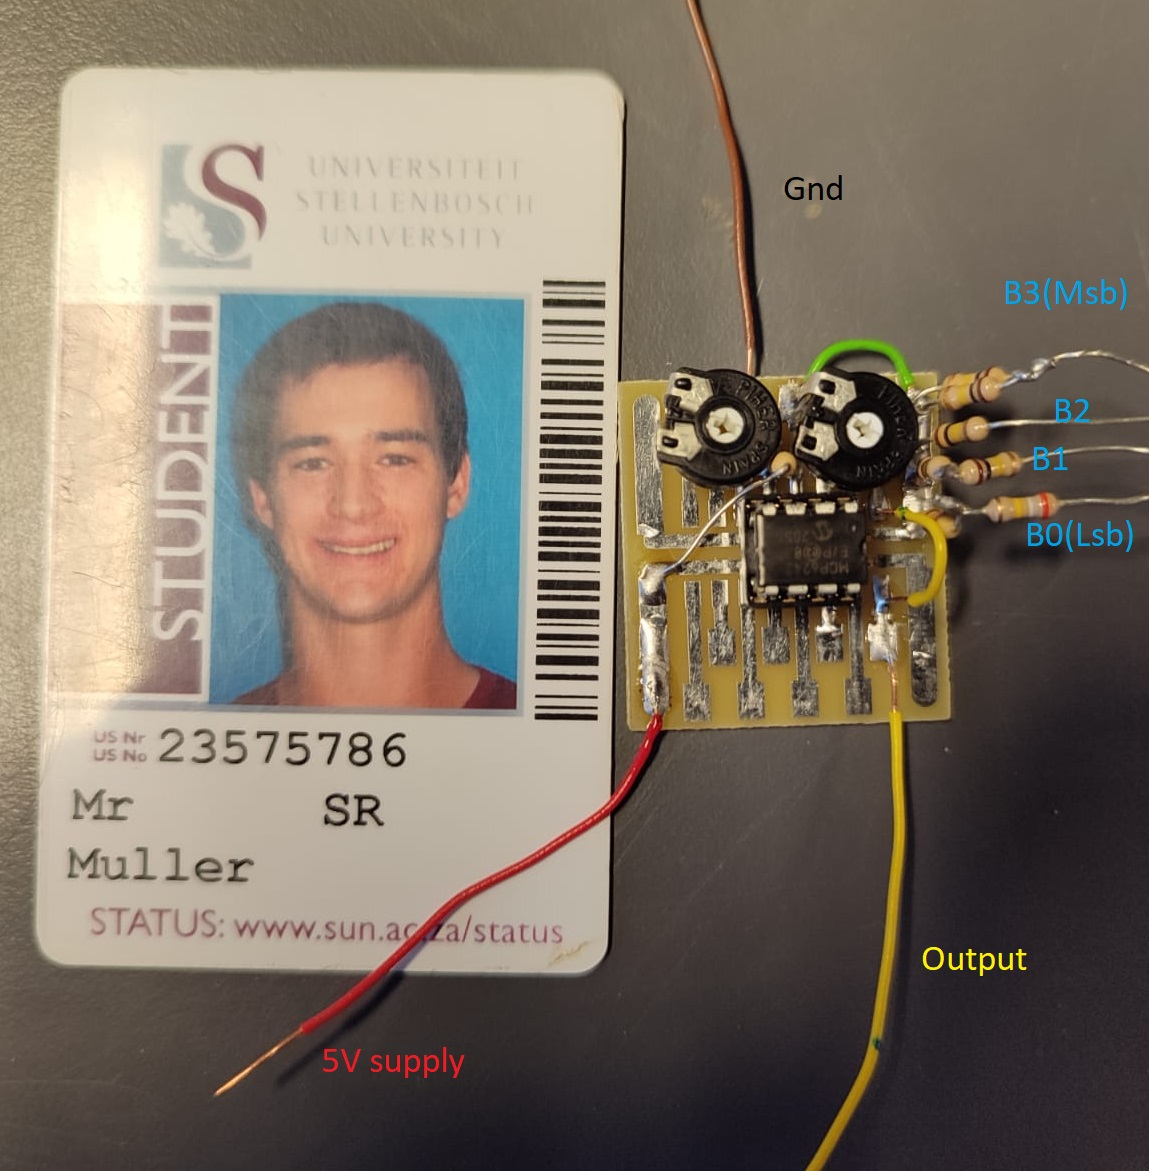
\includegraphics[width = 0.9\textwidth]{./Figures/DAC_Cir_Card.jpeg}
\caption{Labelled circuit and student card for the DAC.}
\label{fig:sonicsen_cir_card}
\end{figure}
\include{Chapter4}
\include{Chapter5}
\include{Chapter6}


% Bibliography
\bibliography{References}

% End matter
\appendix
\chapter{Social contract}
\makeatletter\@mkboth{}{Appendix}\makeatother
\label{appen:social_contract}
     \begin{figure}[!htb]
     \centering
     	\fbox{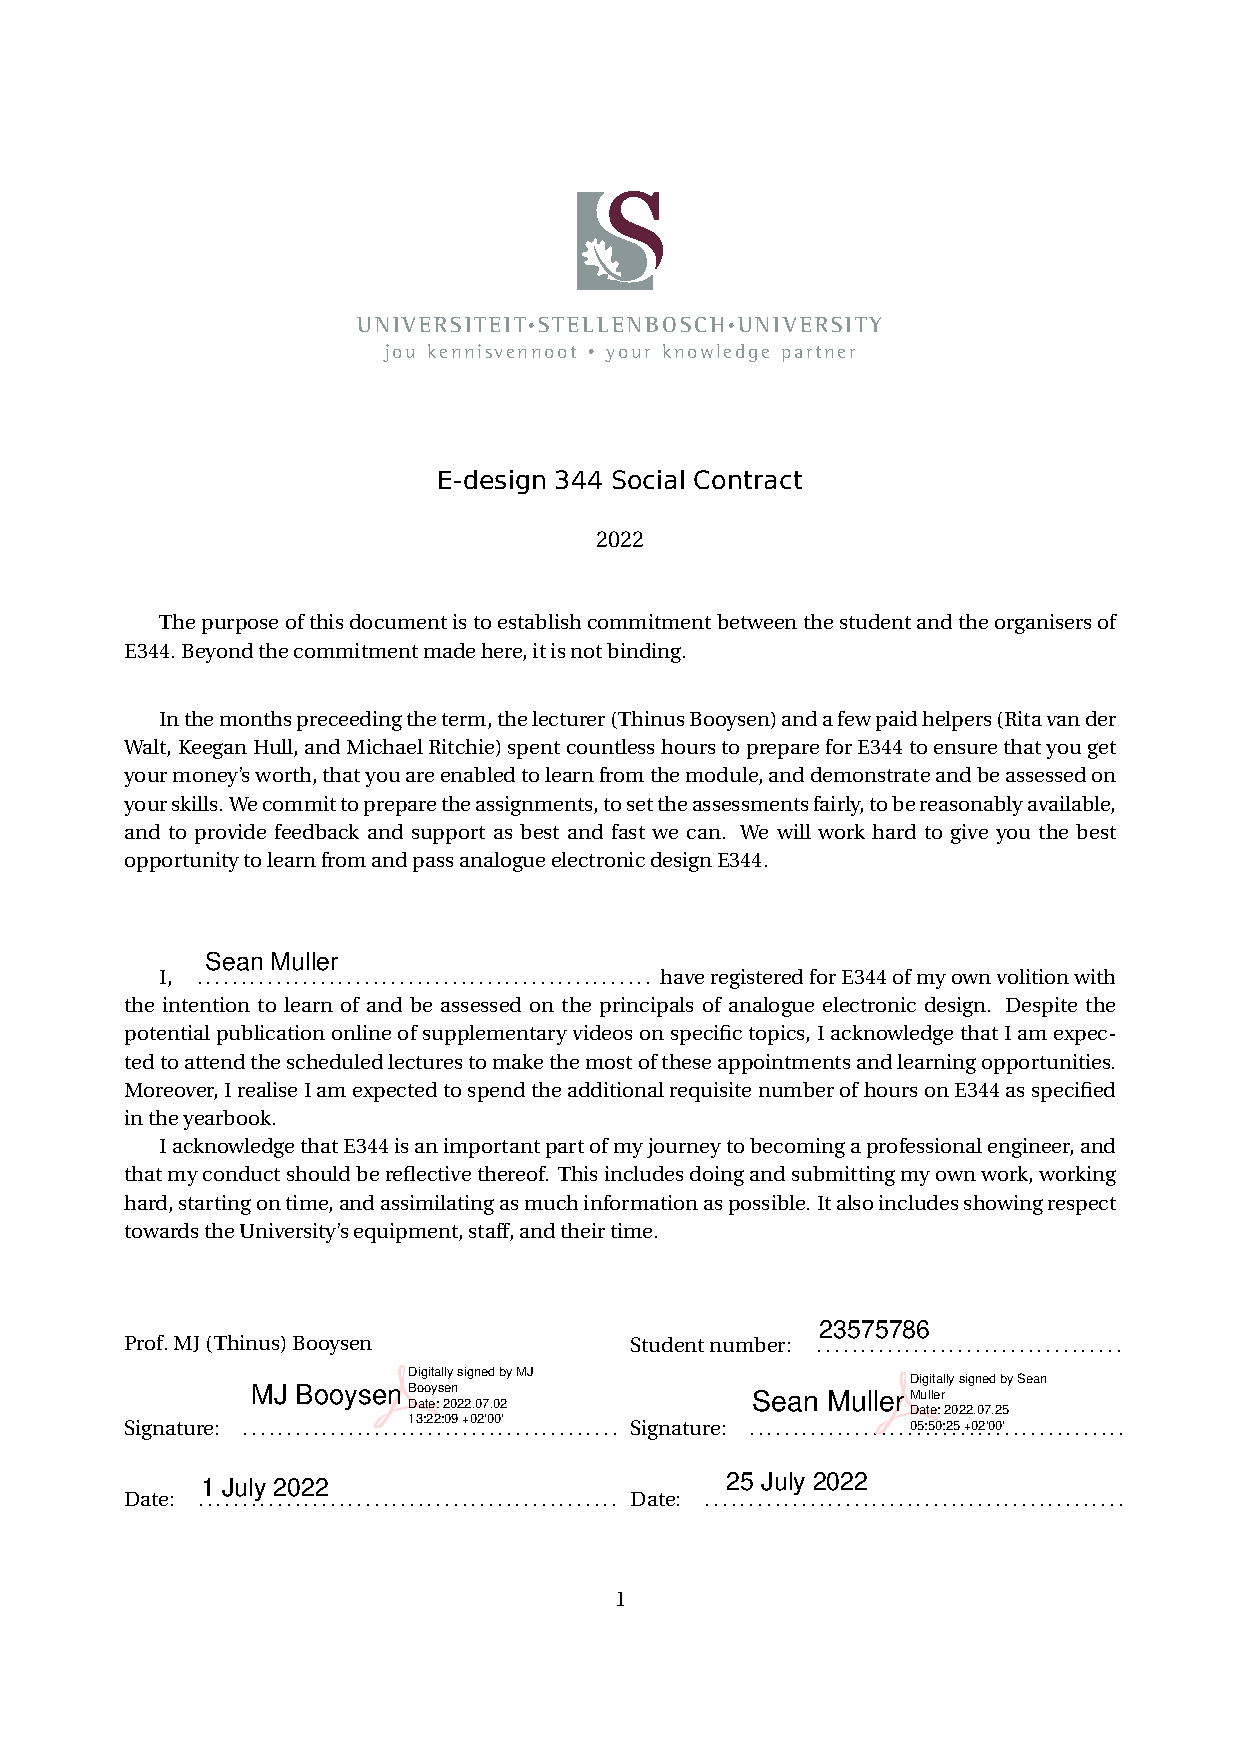
\includegraphics[width=0.8\linewidth]{./Figures/SocialContract_signed.pdf}}
       \label{fig:social_contract}
	\end{figure}
\chapter{GitHub Activity Heatmap}
\makeatletter\@mkboth{}{Appendix}\makeatother
\label{appen:github_heatmap}
\textcolor{red}{Take a screenshot of your github version control activity heatmap and insert here. }

     \begin{figure}[!htb]
     \centering
     	\fbox{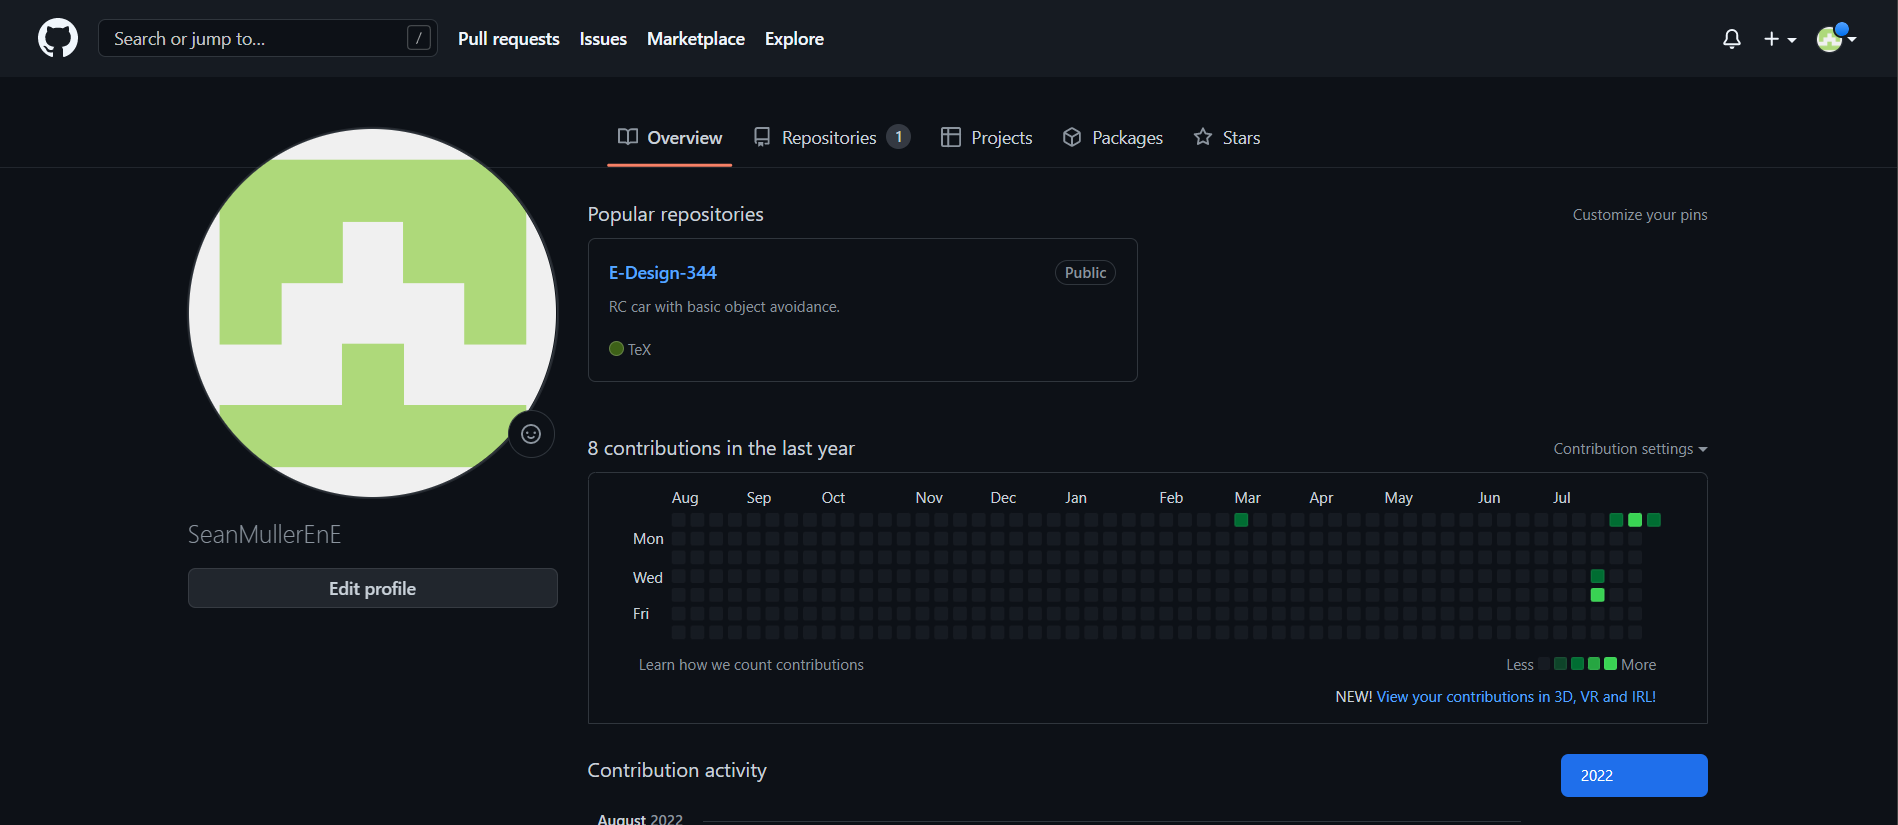
\includegraphics[width=1\linewidth]{./Figures/GitHub.png}}
	\label{fig:github}
	\end{figure}

\end{document}

